\documentclass[12pt,a4paper]{article}
\usepackage[T1]{fontenc}
\usepackage[utf8]{inputenc}
\usepackage{lmodern}
\usepackage{amsmath,amssymb,amsthm,mathtools}
\usepackage{geometry}
\geometry{margin=1in}
\usepackage{microtype}
\usepackage{hyperref}
\usepackage{xcolor}
\usepackage{enumitem}
\usepackage{fancyhdr}
\usepackage{bookmark}

\usepackage{tikz}
\usetikzlibrary{calc,positioning}

\usepackage{centernot}

\usepackage{tikz-cd}

\usepackage{tocloft}
\setlength{\cftsubsecnumwidth}{3.2em}

\hypersetup{
	colorlinks=true,
	linkcolor=blue!50!black,
	urlcolor=blue!50!black,
	citecolor=blue!50!black,
	pdftitle={Theory of Commutative Algebra 7},
	pdfauthor={},
	pdfsubject={Solved problems and theory notes in commutative algebra},
	pdfcreator={OpenAI}
}

\setlist[itemize]{topsep=4pt,itemsep=2pt,parsep=0pt,partopsep=0pt}
\setlength{\parskip}{0.55em}
\setlength{\parindent}{0pt}

\setcounter{secnumdepth}{2}


\setcounter{tocdepth}{2}

\pagestyle{fancy}


\fancyhf{}
\lhead{Theory of Algebraic Topology 2}
\rhead{\thepage}
\renewcommand{\headrulewidth}{0.4pt}

\newtheoremstyle{notespace}{6pt}{6pt}{\normalfont}{} {\bfseries}{.}{0.5em}{}
\theoremstyle{notespace}
\newtheorem{definition}{Definition}[section]
\newtheorem{remark}{Remark}[section]

\DeclareMathOperator{\Spec}{Spec}
\DeclareMathOperator{\Ass}{Ass}
\DeclareMathOperator{\Ann}{Ann}
\DeclareMathOperator{\Supp}{Supp}
\DeclareMathOperator{\Hom}{Hom}
\DeclareMathOperator{\Min}{Min}
\DeclareMathOperator{\Ker}{Ker}
\DeclareMathOperator{\Frac}{Frac}

\DeclareMathOperator{\depth}{depth}
\DeclareMathOperator{\Tor}{Tor}
\DeclareMathOperator{\Ext}{Ext}

\DeclareMathOperator{\coker}{coker}
\DeclareMathOperator{\im}{im}


\title{\vspace{-1.5em}\bfseries Theory of Algebraic Topology 2}
\author{}
\date{\today}

\begin{document}
	\maketitle
	\thispagestyle{plain}
		\begin{center}
		\begin{minipage}{0.92\textwidth}
			Lecture notes with worked examples in algebraic topology
		\end{minipage}
	\end{center}
		\pdfbookmark[1]{Contents}{contents}\tableofcontents
	\clearpage

\section{Attaching cells, homotopic attaching maps, and the dunce cap}

\subsection{Problem 9: Attaching an \(n\)-cell along a map}

Let
\[
f:S^{n-1}\to X
\]
be a continuous map. The space obtained by attaching an \(n\)-cell to \(X\) along \(f\) is defined to be the quotient space
\[
X\cup_f D^n := (X\sqcup D^n)/\sim,
\]
where \(\sim\) is the smallest equivalence relation such that
\[
b\sim f(b)
\qquad
\text{for every } b\in \partial D^n=S^{n-1}.
\]

We want to show:

\medskip

If
\[
f,f':S^{n-1}\to X
\]
are homotopic, then
\[
X\cup_f D^n \simeq X\cup_{f'} D^n.
\]

\subsubsection{What this quotient means}

The quotient
\[
(X\sqcup D^n)/\sim
\]
means that we begin with two disjoint pieces:

\begin{itemize}
	\item the space \(X\),
	\item an \(n\)-disk \(D^n\),
\end{itemize}

and then we glue each boundary point
\[
b\in \partial D^n=S^{n-1}
\]
to the point
\[
f(b)\in X.
\]

So the interior of the disk is new, but the boundary is attached to \(X\) according to the rule given by \(f\).

This is one of the basic constructions in CW-complex theory.

\subsubsection{Intuition}

The boundary sphere
\[
S^{n-1}=\partial D^n
\]
is the place where the new cell is attached. The map \(f\) tells us exactly how the boundary winds around inside \(X\).

The theorem says that the homotopy type of the attached space depends only on the homotopy class of \(f\), not on the particular representative.

So if we continuously deform the attaching map, the resulting attached space changes only up to homotopy equivalence.

\subsubsection{Basic examples of cell attachment}

\paragraph{Example 1: Attach a 1-cell to two points.}
Let
\[
X=\{p,q\},
\]
and let
\[
f:S^0=\{-1,1\}\to X
\]
send one point to \(p\) and the other to \(q\). Then
\[
X\cup_f D^1
\]
is just an interval joining \(p\) to \(q\).

\paragraph{Example 2: Attach a 1-cell to one point.}
Let
\[
X=\{p\},
\]
and let
\[
f:S^0\to X
\]
send both boundary points of \(D^1\) to \(p\). Then
\[
X\cup_f D^1
\]
is a circle:
\[
X\cup_f D^1 \cong S^1.
\]

\paragraph{Example 3: Attach a 2-cell to a point.}
Let
\[
X=\{p\},
\]
and let
\[
f:S^1\to X
\]
be the constant map. Then the whole boundary of the 2-disk is collapsed to one point, so
\[
X\cup_f D^2 \cong D^2/\partial D^2 \cong S^2.
\]

\paragraph{Example 4: Attach a 2-cell to \(S^1\) by the identity.}
Let
\[
X=S^1,
\qquad
f=\mathrm{id}_{S^1}.
\]
Then attaching \(D^2\) along the identity simply fills in the circle. Hence
\[
S^1\cup_{\mathrm{id}} D^2 \cong D^2.
\]

\paragraph{Example 5: Attach a 2-cell to \(S^1\) by a degree \(m\) map.}
Let
\[
f:S^1\to S^1,
\qquad
f(z)=z^m.
\]
Then
\[
S^1\cup_f D^2
\]
is the standard 2-dimensional CW-complex with one 1-cell and one 2-cell attached by degree \(m\). Its fundamental group is
\[
\pi_1(S^1\cup_f D^2)\cong \mathbb{Z}/m\mathbb{Z}.
\]
For \(m=1\), the space is contractible; for \(m=0\), it is homotopy equivalent to
\[
S^1\vee S^2.
\]

\subsubsection{The theorem}

\paragraph{Theorem.}
If
\[
f,f':S^{n-1}\to X
\]
are homotopic, then
\[
X\cup_f D^n \simeq X\cup_{f'} D^n.
\]

\paragraph{\textbf{Solution.}}
Assume
\[
H:S^{n-1}\times[0,1]\to X
\]
is a homotopy from \(f\) to \(f'\), so that
\[
H(u,0)=f(u),
\qquad
H(u,1)=f'(u)
\qquad
\text{for all }u\in S^{n-1}.
\]

We will construct explicit maps
\[
\Phi:X\cup_f D^n \to X\cup_{f'} D^n
\]
and
\[
\Psi:X\cup_{f'} D^n \to X\cup_f D^n
\]
that are homotopy inverses.

\medskip

Write points of \(D^n\) in polar form
\[
ru,
\qquad
0\le r\le 1,
\qquad
u\in S^{n-1}.
\]

Define
\[
\Phi:X\cup_f D^n \to X\cup_{f'} D^n
\]
as follows.

On \(X\), let
\[
\Phi(x)=x.
\]

On the attached disk \(D^n\), define
\[
\Phi(ru)=
\begin{cases}
	2ru, & 0\le r\le \dfrac12,\\[1.2ex]
	H\bigl(u,\,2-2r\bigr), & \dfrac12\le r\le 1.
\end{cases}
\]

Here the first case is interpreted as a point of the attached disk in
\[
X\cup_{f'} D^n,
\]
while the second case is interpreted as a point of \(X\).

We check the compatibility.

At
\[
r=\frac12,
\]
the first formula gives the boundary point
\[
u\in \partial D^n,
\]
which in the quotient \(X\cup_{f'} D^n\) is identified with
\[
f'(u)=H(u,1).
\]
The second formula at \(r=\frac12\) gives exactly
\[
H(u,1)=f'(u).
\]
So the two formulas agree.

At
\[
r=1,
\]
the second formula gives
\[
H(u,0)=f(u).
\]
But in the source quotient \(X\cup_f D^n\), the boundary point \(u\in \partial D^n\) is identified with \(f(u)\in X\). Therefore the definition is well defined on the quotient.

Thus \(\Phi\) is continuous and well defined.

\medskip

Now define
\[
\Psi:X\cup_{f'} D^n \to X\cup_f D^n
\]
in the same way but using the reverse homotopy
\[
\widetilde{H}(u,t)=H(u,1-t),
\]
which runs from \(f'\) to \(f\). So on \(X\),
\[
\Psi(x)=x,
\]
and on the attached disk,
\[
\Psi(ru)=
\begin{cases}
	2ru, & 0\le r\le \dfrac12,\\[1.2ex]
	\widetilde{H}\bigl(u,\,2-2r\bigr), & \dfrac12\le r\le 1.
\end{cases}
\]

Again \(\Psi\) is continuous and well defined.

\medskip

We now explain why \(\Phi\) and \(\Psi\) are homotopy inverses.

The composite
\[
\Psi\circ \Phi
\]
fixes \(X\), and on the disk it first pushes the outer annulus across the homotopy from \(f\) to \(f'\), then pushes it back from \(f'\) to \(f\). Geometrically, this simply shrinks the annulus and then expands it again, so it is homotopic to the identity map on
\[
X\cup_f D^n.
\]

Likewise,
\[
\Phi\circ \Psi
\]
is homotopic to the identity on
\[
X\cup_{f'} D^n.
\]

Hence
\[
\Phi
\quad\text{and}\quad
\Psi
\]
are homotopy inverses, and therefore
\[
X\cup_f D^n \simeq X\cup_{f'} D^n.
\]

\paragraph{Conclusion.}
The homotopy type of the space obtained by attaching an \(n\)-cell depends only on the homotopy class of the attaching map
\[
f:S^{n-1}\to X.
\]

\subsection{Problem 10: The dunce cap}

The \emph{dunce cap} is the space obtained from a solid triangle by gluing the three boundary edges together according to the directions indicated in the picture.

We want to show that this space is contractible.

\subsubsection{Intuition}

The key idea is that the dunce cap is a 2-cell attached to a circle by a map of degree
\[
\pm 1.
\]
A degree \(\pm 1\) map
\[
S^1\to S^1
\]
is homotopic to a homeomorphism of the circle. By Problem 9, attaching along this map gives a space homotopy equivalent to attaching along a homeomorphism. But attaching a 2-cell along a homeomorphism simply gives a disk, and a disk is contractible.

So the whole argument is:

\[
\text{dunce cap}
\sim
\text{attach }D^2\text{ to }S^1\text{ by degree }\pm1
\sim
\text{attach }D^2\text{ by a homeomorphism}
\cong
D^2.
\]

\subsubsection{Step 1: The boundary identifications produce a circle}

Let \(\Delta^2\) be the solid triangle. First look only at its boundary \(\partial \Delta^2\).

Under the prescribed identifications, all three edges are glued together to one 1-cell. The three vertices are also all identified to one point. Therefore the quotient of the boundary is a CW-complex with:

\begin{itemize}
	\item one 0-cell,
	\item one 1-cell.
\end{itemize}

Hence the quotient of the boundary is homeomorphic to
\[
S^1.
\]

So the dunce cap may be viewed as a space obtained by attaching the interior 2-cell of the triangle to a circle.

\subsubsection{Step 2: The attaching map has degree \(\pm1\)}

Let us denote by \(a\) the unique oriented 1-cell in the boundary quotient.

Now traverse the boundary of the triangle once. Because of the arrow directions in the picture, one side is traversed in the same direction as \(a\), while the other two sides are traversed in the opposite direction. Therefore the attaching word is, up to cyclic permutation,
\[
a\,a^{-1}\,a^{-1},
\]
or equivalently the exponent sum is
\[
1-1-1=-1.
\]

If we choose the opposite orientation of the boundary, the exponent sum becomes
\[
1.
\]

Thus the attaching map
\[
g:S^1\to S^1
\]
has degree
\[
\deg(g)=\pm1.
\]

The sign is not important for contractibility; what matters is that the degree is \(\pm1\).

\subsubsection{Step 3: Replace the attaching map by a homeomorphism}

Any map
\[
g:S^1\to S^1
\]
of degree \(1\) is homotopic to the identity map, and any map of degree \(-1\) is homotopic to a reflection. In either case, \(g\) is homotopic to a homeomorphism
\[
h:S^1\to S^1.
\]

By Problem 9,
\[
S^1\cup_g D^2 \simeq S^1\cup_h D^2.
\]

But attaching a 2-cell to \(S^1\) by a homeomorphism simply fills in the circle, so
\[
S^1\cup_h D^2 \cong D^2.
\]

Therefore
\[
S^1\cup_g D^2 \simeq D^2.
\]

Since \(D^2\) is contractible, it follows that the dunce cap is contractible.

\subsubsection{Formal proof}

\paragraph{\textbf{Solution.}}
Let \(D\) denote the dunce cap. By the edge identifications, the quotient of the boundary of the triangle is a circle:
\[
\partial \Delta^2/\!\sim \;\cong S^1.
\]
Hence \(D\) can be written as
\[
D \cong S^1\cup_g D^2
\]
for some attaching map
\[
g:S^1\to S^1.
\]

Reading the boundary according to the arrows shows that the total winding number of \(g\) around the unique circle is
\[
\deg(g)=\pm1.
\]
Therefore \(g\) is homotopic to a homeomorphism
\[
h:S^1\to S^1.
\]

By Problem 9,
\[
S^1\cup_g D^2 \simeq S^1\cup_h D^2.
\]
Since \(h\) is a homeomorphism, attaching \(D^2\) along \(h\) yields a disk:
\[
S^1\cup_h D^2 \cong D^2.
\]
Thus
\[
D \simeq D^2.
\]
Because \(D^2\) is contractible, the dunce cap is contractible.

\paragraph{Conclusion.}
The dunce cap is contractible.

\subsubsection{Remark}

The dunce cap is a famous example because it is contractible but not collapsible. Thus it is topologically trivial from the homotopy point of view, but combinatorially quite subtle.

\subsection{Summary of the two problems}

Problem 9 tells us that in a cell attachment
\[
X\cup_f D^n,
\]
only the homotopy class of the attaching map \(f\) matters up to homotopy equivalence.

Problem 10 uses this principle in a concrete and nontrivial example: the dunce cap is built by attaching a 2-cell to \(S^1\), and the attaching map has degree \(\pm1\). Hence it is homotopic to a homeomorphism of \(S^1\), so the resulting space is homotopy equivalent to a disk and therefore contractible.

\subsection{The quotient \(X\cup_f D^n=(X\sqcup D^n)/\sim\): meaning, construction, and examples}

Let
\[
f:S^{n-1}\to X
\]
be a continuous map. The space obtained by attaching an \(n\)-cell to \(X\) along \(f\) is defined by
\[
X\cup_f D^n := (X\sqcup D^n)/\sim,
\]
where \(\sim\) is the smallest equivalence relation such that
\[
b\sim f(b)
\qquad
\text{for every } b\in \partial D^n=S^{n-1}.
\]

This subsection explains carefully what this quotient means.

\subsubsection{Step 1: Start with a disjoint union}

The notation
\[
X\sqcup D^n
\]
means the \emph{disjoint union} of \(X\) and the disk \(D^n\).

So at the beginning, the space consists of two completely separate pieces:

\[
X
\qquad\text{and}\qquad
D^n.
\]

No point of \(X\) is equal to any point of \(D^n\), even if they might look similar as sets. In a disjoint union, we keep the two spaces separate.

\subsubsection{Step 2: Identify boundary points of the disk with points of \(X\)}

The boundary of the disk is
\[
\partial D^n=S^{n-1}.
\]
The map
\[
f:S^{n-1}\to X
\]
tells us where each boundary point of the disk is supposed to be attached in \(X\).

Thus for each point
\[
b\in \partial D^n,
\]
we impose the relation
\[
b\sim f(b).
\]

In words:

\begin{quote}
	Each boundary point of the disk is glued to the point of \(X\) specified by the attaching map \(f\).
\end{quote}

Only these identifications are forced. Interior points of the disk are not identified with points of \(X\); they remain new points of the attached cell.

\subsubsection{Step 3: The phrase ``smallest equivalence relation''}

The relation \(\sim\) must be an equivalence relation, so it must satisfy:

\begin{itemize}
	\item reflexivity,
	\item symmetry,
	\item transitivity.
\end{itemize}

We begin with the basic identifications
\[
b\sim f(b)
\qquad
(b\in \partial D^n),
\]
and then enlarge this relation only as much as necessary so that it becomes an equivalence relation.

This is what is meant by the \emph{smallest equivalence relation containing} those identifications.

\subsubsection{Step 4: The quotient space}

The quotient
\[
(X\sqcup D^n)/\sim
\]
is the set of equivalence classes for this relation, equipped with the quotient topology.

The quotient map is
\[
q:X\sqcup D^n\to (X\sqcup D^n)/\sim.
\]

A subset
\[
U\subset (X\sqcup D^n)/\sim
\]
is open if and only if
\[
q^{-1}(U)
\]
is open in \(X\sqcup D^n\).

So the quotient topology is exactly the topology obtained after performing the prescribed gluing.

\subsubsection{Geometric picture}

The construction
\[
X\cup_f D^n
\]
should be visualized as follows:

\begin{enumerate}
	\item take the old space \(X\),
	\item take a new disk \(D^n\),
	\item glue the boundary sphere \(\partial D^n=S^{n-1}\) to \(X\) via the map \(f\),
	\item keep the interior of the disk as genuinely new points.
\end{enumerate}

Thus \(X\cup_f D^n\) is obtained by \emph{attaching} the disk \(D^n\) to \(X\) along its boundary.

\subsubsection{What remains unchanged and what gets glued}

It is important to distinguish three kinds of points.

\paragraph{Points of \(X\).}
These remain in the quotient, although some boundary points of the disk may be identified with them.

\paragraph{Interior points of \(D^n\).}
These are not identified with anything in \(X\). They survive as new points in the quotient.

\paragraph{Boundary points of \(D^n\).}
These are glued onto \(X\) according to the rule
\[
b\sim f(b).
\]

So the boundary of the new cell disappears as a separate boundary and becomes attached to the old space.

\subsubsection{Example 1: Attach an interval to two points}

Let
\[
X=\{p,q\},
\]
and let
\[
f:S^0=\{-1,1\}\to X
\]
be defined by
\[
f(-1)=p,
\qquad
f(1)=q.
\]

Then
\[
X\cup_f D^1 = (\{p,q\}\sqcup D^1)/\sim
\]
with the identifications
\[
-1\sim p,
\qquad
1\sim q.
\]

Geometrically, we take an interval \(D^1=[-1,1]\) and glue its left endpoint to \(p\) and its right endpoint to \(q\). The resulting space is just an interval with endpoints labeled by the two points \(p\) and \(q\). So
\[
X\cup_f D^1 \cong [0,1].
\]

\subsubsection{Example 2: Attach an interval to one point}

Let
\[
X=\{p\},
\]
and let
\[
f:S^0\to X
\]
send both points of \(S^0\) to \(p\):
\[
f(-1)=p,
\qquad
f(1)=p.
\]

Then
\[
X\cup_f D^1
=
(\{p\}\sqcup [-1,1])/\sim
\]
with
\[
-1\sim p,
\qquad
1\sim p.
\]

So both endpoints of the interval are glued to the same point. This produces a circle:
\[
X\cup_f D^1 \cong S^1.
\]

This is one of the simplest and most important quotient constructions in topology.

\subsubsection{Example 3: Attach a 2-cell to a point}

Let
\[
X=\{p\},
\]
and let
\[
f:S^1\to X
\]
be the constant map:
\[
f(z)=p
\qquad
\text{for all } z\in S^1.
\]

Then
\[
X\cup_f D^2
=
(\{p\}\sqcup D^2)/\sim
\]
where every boundary point of the disk is identified with \(p\). Thus the whole boundary \(\partial D^2=S^1\) is collapsed to one point.

So
\[
X\cup_f D^2 \cong D^2/\partial D^2 \cong S^2.
\]

Thus a 2-sphere can be described as a 2-disk whose boundary is collapsed to a point.

\subsubsection{Example 4: Attach a 2-cell to a circle by the identity}

Let
\[
X=S^1,
\qquad
f=\mathrm{id}_{S^1}.
\]

Then
\[
X\cup_f D^2=(S^1\sqcup D^2)/\sim
\]
with
\[
b\sim b
\qquad
\text{for } b\in S^1=\partial D^2.
\]

So the boundary of the disk is glued to the circle in the obvious way. Geometrically, this simply fills the circle with a disk. Therefore
\[
S^1\cup_{\mathrm{id}} D^2 \cong D^2.
\]

\subsubsection{Example 5: Attach a disk by a constant map}

Let
\[
X=S^1,
\]
and let
\[
f:S^1\to S^1
\]
be constant.

Then every boundary point of the new disk is attached to one single point of \(X\). So the new 2-cell contributes a sphere attached at one point to the original circle. The resulting space is homotopy equivalent, and in fact homeomorphic as a quotient, to
\[
S^1\vee S^2,
\]
the wedge of a circle and a sphere.

This is a good example showing that the quotient depends strongly on the attaching map \(f\).

\subsubsection{Example 6: General viewpoint for CW-complexes}

In CW-complex language, the space
\[
X\cup_f D^n
\]
is obtained from \(X\) by adding one \(n\)-cell.

The old space \(X\) is the \((n-1)\)-skeleton part already built, and the map
\[
f:S^{n-1}\to X
\]
is the attaching map telling us how the boundary of the new cell is glued to the old space.

So the quotient notation is not just formal symbolism: it is the precise way of encoding cell attachment.

\subsubsection{Why the quotient is necessary}

Without quotient notation, it would be difficult to express gluing rigorously.

If we only wrote ``glue \(\partial D^n\) to \(X\) by \(f\),'' this would be geometrically intuitive but not formally precise. The quotient
\[
(X\sqcup D^n)/\sim
\]
gives an exact set-theoretic and topological definition of the glued space.

Thus quotient spaces are the standard language for constructions where points are identified.

\subsubsection{A useful way to think about the quotient map}

The quotient map
\[
q:X\sqcup D^n\to X\cup_f D^n
\]
has the following behavior:

\begin{itemize}
	\item on interior points of \(D^n\), it is injective,
	\item on points of \(X\), it is injective unless some boundary points of \(D^n\) are also mapped there,
	\item on the boundary \(\partial D^n\), it identifies each \(b\) with \(f(b)\in X\).
\end{itemize}

So the only nontrivial collapsing occurs exactly on the boundary of the cell.

\subsubsection{What \(X\cup_f D^n\) is \emph{not}}

It is important not to confuse
\[
X\cup_f D^n
\]
with the ordinary union \(X\cup D^n\) inside some ambient space. Usually \(X\) and \(D^n\) are not already sitting inside one larger space in the right way. The quotient construction creates the glued space abstractly.

It is also not just a disjoint union:
\[
X\cup_f D^n \neq X\sqcup D^n,
\]
because the boundary points of the disk are identified with points of \(X\).

\subsubsection{Final summary}

The quotient
\[
X\cup_f D^n=(X\sqcup D^n)/\sim
\]
means:

\begin{quote}
	Take the old space \(X\), take a new disk \(D^n\), and glue every boundary point
	\[
	b\in \partial D^n=S^{n-1}
	\]
	to the point
	\[
	f(b)\in X.
	\]
	The result is a new space in which the interior of the disk becomes a new \(n\)-dimensional cell attached to \(X\).
\end{quote}

So the quotient formalizes the geometric act of attaching a cell, and it is one of the fundamental constructions in algebraic topology.

\subsection{What the dunce cap looks like}

The \emph{dunce cap} is not a cap in the ordinary geometric sense, and it is not a smooth surface sitting nicely in \(\mathbb{R}^3\). Instead, it is a \emph{quotient space} obtained from a solid triangle by identifying its boundary edges in a particular way.

\subsubsection{The starting point}

Begin with a filled triangle
\[
\Delta^2.
\]
So before any identifications are made, we simply have an ordinary 2-dimensional disk with polygonal boundary.

The triangle has:

\begin{itemize}
	\item three vertices,
	\item three edges,
	\item one 2-dimensional interior.
\end{itemize}

\subsubsection{The gluing rule}

Now orient the three boundary edges as indicated by arrows in the standard picture of the dunce cap. Then identify the three edges with each other according to those directions.

This means:

\begin{itemize}
	\item all three edges are glued into one single edge,
	\item all three vertices are identified to one single point,
	\item the interior of the triangle remains as one 2-cell.
\end{itemize}

So after gluing, the resulting space has the structure of a CW-complex with:

\[
\text{one 0-cell, one 1-cell, and one 2-cell.}
\]

\subsubsection{Why it is hard to picture directly}

The dunce cap is difficult to draw faithfully as an ordinary object in the plane or in 3-dimensional space, because the quotient identifications force different parts of the boundary to occupy the same place.

Thus the usual picture is not a literal drawing of the final space. Instead, one normally draws:

\begin{itemize}
	\item a triangle,
	\item arrows on the edges,
	\item and understands the picture as an instruction for gluing.
\end{itemize}

So the standard diagram should be read as:

\begin{quote}
	Take this triangle and glue its boundary edges together according to the arrow directions.
\end{quote}

\subsubsection{A verbal description of the final space}

Topologically, the dunce cap looks like:

\begin{itemize}
	\item one single vertex,
	\item one loop-like edge,
	\item one 2-dimensional face attached along that edge.
\end{itemize}

However, the attaching is not the ordinary one that produces a disk. The same edge is traced several times by the boundary of the face, with the orientations prescribed by the arrows. This makes the quotient highly singular from a geometric point of view, even though it turns out to be contractible.

So the dunce cap should be imagined as:

\begin{quote}
	a solid triangle whose entire boundary has been folded and glued onto a single edge in a nontrivial way.
\end{quote}

\subsubsection{What happens to the vertices and edges}

Let the boundary of the triangle consist of three edges
\[
e_1,\quad e_2,\quad e_3.
\]
After the identifications:

\begin{itemize}
	\item the three vertices of the triangle become one point,
	\item the three edges become one edge,
	\item the interior remains one 2-cell attached to that edge.
\end{itemize}

Thus the quotient is much smaller combinatorially than the original triangle, but the way the boundary wraps onto the single edge is nontrivial.

\subsubsection{Why the name can be misleading}

The phrase ``dunce cap'' is historical. It should not suggest that the space is literally shaped like a cone or hat. The name refers to the standard pedagogical nickname for this quotient space, not to its ordinary geometric appearance.

From the topological point of view, it is best understood as a quotient of a triangle, not as a familiar surface.

\subsubsection{A useful mental image}

A good mental model is the following:

\begin{enumerate}
	\item take a paper triangle,
	\item mark arrows on the edges,
	\item glue the three edges together according to those arrows,
	\item let the interior of the triangle remain filled in.
\end{enumerate}

The result is the dunce cap.

Although the space is contractible, it is not geometrically simple in the combinatorial sense. In fact, it is famous because it is contractible but not collapsible.

\subsubsection{Compact summary}

The dunce cap is:

\begin{quote}
	the quotient of a solid triangle obtained by identifying all three boundary edges to one edge, with the identifications prescribed by the arrow directions.
\end{quote}

So, in CW-complex language, it has:

\[
\text{one vertex},\qquad
\text{one edge},\qquad
\text{one 2-cell}.
\]

Its standard picture is not meant to show the final quotient directly, but rather the gluing instructions that define it.

\subsection{Does gluing two edges of a triangle give a cone?}

The short answer is:

\begin{quote}
	Not in general.
\end{quote}

One has to distinguish carefully between:

\begin{itemize}
	\item a triangle \emph{already viewed as a cone},
	\item a quotient obtained by \emph{gluing two edges} of a triangle,
	\item and more singular identifications such as the dunce cap, where \emph{all three} edges are glued together in a special way.
\end{itemize}

\subsubsection{A triangle itself can be viewed as a cone}

A filled triangle \(\Delta^2\) is homeomorphic to a 2-disk \(D^2\). It may also be viewed as the cone on an interval.

Indeed, if
\[
I=[0,1],
\]
then the cone on \(I\) is
\[
CI=(I\times[0,1])/(I\times\{1\}\text{ collapsed to one point}).
\]
Topologically this is a filled triangle: the interval \(I\times\{0\}\) is the base, and the collapsed top
\[
I\times\{1\}
\]
is the apex.

Thus one may say:

\begin{quote}
	A triangle is a cone on one of its edges.
\end{quote}

But this is different from saying:

\begin{quote}
	If we glue two edges of a triangle together, then we obtain a cone.
\end{quote}

That second statement is generally false.

\subsubsection{What gluing two edges means}

Let \(\Delta^2\) be a filled triangle with boundary edges
\[
e_1,\qquad e_2,\qquad e_3.
\]
Suppose we identify \(e_1\) and \(e_2\) by a homeomorphism
\[
\varphi:e_1\to e_2.
\]
Then the quotient space is
\[
\Delta^2/\!\sim,
\]
where
\[
x\sim \varphi(x)
\qquad
\text{for all }x\in e_1.
\]

In this construction:

\begin{itemize}
	\item the interior of the triangle is left unchanged,
	\item the points of \(e_1\) and \(e_2\) are glued together pairwise,
	\item the third edge \(e_3\) remains as part of the boundary.
\end{itemize}

So this quotient identifies two boundary arcs, but it does \emph{not} usually collapse an entire set to one apex. Therefore it is not, in general, a cone construction.

\subsubsection{Why this is different from a cone}

The cone on a space \(X\) is defined by
\[
CX=(X\times[0,1])/(X\times\{1\}\text{ collapsed to one point}).
\]
The crucial feature is that an entire copy of \(X\) is collapsed to a \emph{single point}, the apex.

By contrast, when two edges of a triangle are glued together, points are usually identified \emph{pairwise}, not all collapsed to one point. So the quotient behaves differently.

Thus:

\[
\text{cone} \neq \text{pairwise gluing of two edges}
\]
in general.

\subsubsection{Typical outcome of gluing two edges}

If one glues two edges of a filled triangle together in the usual point-by-point way, the resulting quotient is typically still contractible, and in fact it is often homeomorphic to a disk.

Intuitively, the triangle remains a single 2-cell, and identifying two boundary edges usually creates a seam rather than a genuine cone point.

So a useful informal slogan is:

\begin{quote}
	Gluing two edges of a triangle usually produces a disk-like quotient with an identification seam, not a cone.
\end{quote}

\subsubsection{A simple model example}

Take the square
\[
[0,1]\times[0,1]
\]
and identify two adjacent edges. One may obtain a space that is still contractible and still disk-like, but with boundary points identified. The same phenomenon occurs for triangles: gluing two boundary edges does not automatically create the apex-collapse that defines a cone.

This is why one must be careful not to confuse:

\begin{itemize}
	\item quotient identifications along edges,
	\item with the special quotient that defines a cone.
\end{itemize}

\subsubsection{Why the dunce cap is more complicated}

The dunce cap is obtained by gluing \emph{all three} edges of a triangle together according to a prescribed orientation pattern.

So in the dunce cap:

\begin{itemize}
	\item all three edges become one edge,
	\item all three vertices become one vertex,
	\item the 2-cell is attached in a highly nontrivial way.
\end{itemize}

This is much more singular than merely gluing two edges together. Therefore the dunce cap should not be thought of as ``just a cone'' obtained from a triangle.

\subsubsection{A good way to remember the distinction}

It is helpful to separate the following three statements.

\paragraph{Statement 1.}
A filled triangle is homeomorphic to a disk.

\paragraph{Statement 2.}
A filled triangle may be viewed as the cone on one of its edges.

\paragraph{Statement 3.}
Gluing two edges of a triangle together does \emph{not} in general produce a cone.

The first two are true. The third warns against a common confusion.

\subsubsection{Final summary}

So the correct conclusion is:

\begin{quote}
	A triangle itself can be viewed as a cone on an interval, but gluing two edges of a triangle together does not, in general, give a cone.
\end{quote}

What gluing two edges produces is usually a quotient space with a seam or identification along the boundary, often still disk-like and contractible, but not the cone construction in the strict topological sense.
	

\subsection{Why the arrows matter in edge identifications}

When one draws a polygon or triangle and indicates that certain edges are to be glued together, the arrows on the edges are not decorative. They are an essential part of the data of the quotient construction.

\subsubsection{The basic idea}

Suppose two edges
\[
e_1
\qquad\text{and}\qquad
e_2
\]
are to be identified. To define the quotient precisely, one must specify \emph{how} points of \(e_1\) are matched with points of \(e_2\). The arrows tell us exactly this.

An arrow on an edge gives that edge an \emph{orientation}. Thus the arrows determine whether the identification is:

\begin{itemize}
	\item orientation-preserving, or
	\item orientation-reversing.
\end{itemize}

This can completely change the resulting quotient space.

\subsubsection{What the arrows tell us}

If an edge is traversed in the direction of its arrow, then the arrow tells us which endpoint is the initial point and which endpoint is the terminal point.

When two edges are identified, the arrows tell us which points correspond under the gluing map. In particular, they determine:

\begin{itemize}
	\item which endpoint of one edge is identified with which endpoint of the other,
	\item whether the two edges are glued in the same direction or in opposite directions,
	\item how the boundary of the polygon is read as an attaching map.
\end{itemize}

So the arrows specify the actual quotient map, not merely the fact that some edges are glued.

\subsubsection{Same direction versus opposite direction}

Suppose two edges
\[
e_1,\ e_2
\]
are identified.

\paragraph{Same-direction gluing.}
If the arrows point in corresponding directions, then points are identified while moving along both edges in the same oriented direction.

\paragraph{Opposite-direction gluing.}
If the arrows point in opposite directions, then points are identified while moving along one edge in the reverse order relative to the other.

These two gluings are generally different and often lead to different quotient spaces.

\subsubsection{Why this matters topologically}

Changing the direction of an edge identification can change:

\begin{itemize}
	\item which vertices become identified,
	\item the word read along the boundary of a cell,
	\item the degree or homotopy class of the attaching map,
	\item and in many cases the homeomorphism type of the quotient.
\end{itemize}

So the arrows influence the topology of the final space, not just the way the picture is drawn.

\subsubsection{A familiar polygon example}

This phenomenon already appears in the classification of surfaces.

For a square, if one glues opposite edges with matching orientations, one obtains a torus. If one changes one of the directions, one gets a different quotient, such as the Klein bottle after a suitable pattern of identifications.

Thus the arrows matter because they record the orientation data of the gluing.

\subsubsection{Why the arrows matter for the dunce cap}

In the dunce cap, all three edges of a triangle are identified to one edge, but not arbitrarily. The arrows prescribe the precise way in which the boundary of the triangle wraps around that single edge.

So the arrows determine the attaching map
\[
S^1\to S^1
\]
of the 2-cell. If the arrow pattern is changed, then the attaching map changes, and this may alter the resulting quotient space.

Therefore, for the dunce cap, the arrows are part of the definition of the space.

\subsubsection{The attaching word viewpoint}

When one walks once around the boundary of a polygon, the arrows allow one to record a word in the edge symbols and their inverses.

If an edge is traversed in the direction of its arrow, one records the symbol
\[
a.
\]
If it is traversed opposite to the arrow, one records
\[
a^{-1}.
\]

Thus the arrows determine the boundary word. That word describes the attaching map of the 2-cell and therefore the quotient space itself.

So the arrows do not merely indicate direction visually; they encode the algebraic and topological content of the gluing.

\subsubsection{A simple triangle example}

Suppose two edges of a triangle are glued together.

If the arrows are chosen one way, then one pair of vertices may be identified first and the third edge may remain attached in a certain pattern. If the arrows are reversed, the vertex identifications may change, and the quotient may be different.

So even in the simplest triangle-edge identification, the arrows determine the precise quotient relation.

\subsubsection{The quotient-map interpretation}

From the quotient-space point of view, arrows specify the gluing homeomorphism
\[
\varphi:e_1\to e_2.
\]
Without arrows, we would know only that the edges are to be identified, but not which point of \(e_1\) corresponds to which point of \(e_2\).

Thus the arrows are exactly what turns an informal picture into a well-defined quotient.

\subsubsection{Final summary}

The arrows on edges have genuine mathematical meaning.

\begin{quote}
	They determine the gluing map, the orientation of the identification, the induced boundary word, and therefore the topology of the quotient space.
\end{quote}

In particular, for spaces such as the dunce cap, the arrows are not optional decoration. They are part of the data that defines the space.

\subsection{Two natural meanings of ``gluing one edge of a triangle''}

The phrase ``gluing one edge of a triangle'' is ambiguous. There are at least two natural quotient constructions one might mean, and they lead to different spaces.

\subsubsection{Case 1: Collapse one whole edge to a point}

Let \(\Delta^2\) be a filled triangle, and let
\[
e\subset \partial \Delta^2
\]
be one of its boundary edges. Consider the quotient
\[
\Delta^2/e,
\]
meaning that all points of the edge \(e\) are identified to a single point.

\paragraph{Geometric intuition.}
In a picture, this quotient may look like a pinched disk, or like a cigar with one sharp end. The whole chosen edge is shrunk down to one point, while the rest of the triangle remains present.

\paragraph{Topological meaning.}
Although the picture looks singular, the resulting space is still homeomorphic to a disk:
\[
\Delta^2/e \cong D^2.
\]

\paragraph{Reason.}
A triangle is already homeomorphic to a disk, and collapsing one boundary edge does not create a hole or new essential loop. It only pinches part of the boundary. Thus the quotient remains contractible and disk-like.

So this construction may \emph{look} cigar-like, but topologically it is just a 2-disk.

\subsubsection{Case 2: Identify the two endpoints of one edge}

Now let
\[
e=[v_1,v_2]
\]
be one edge of the triangle, and impose only the relation
\[
v_1\sim v_2.
\]
So the entire edge is \emph{not} collapsed; only its two endpoints are identified.

\paragraph{Geometric intuition.}
The edge \(e\) now becomes a loop based at the identified vertex. The triangle interior is still present, but the boundary has been modified in a nontrivial way.

\paragraph{Topological meaning.}
This quotient is no longer simply an ordinary disk. Identifying the endpoints of one boundary edge creates a genuine circular feature in the boundary quotient.

A good way to think about it is that the boundary now contains a loop, and the interior 2-cell is attached to that quotient boundary. So the result is very different from the previous case.

\paragraph{Comparison with Case 1.}
In Case 1, the whole edge disappears into one point, and the quotient is still a disk. In Case 2, the edge remains but its endpoints are glued together, so the quotient acquires a loop-like feature and is topologically more interesting.

\subsubsection{Why the two constructions are different}

These two quotients are fundamentally different because:

\begin{itemize}
	\item in Case 1, an entire interval is collapsed to one point;
	\item in Case 2, only the two endpoints are identified, while the interior of the edge survives.
\end{itemize}

Thus they should not be confused.

\subsubsection{Final summary}

So the phrase ``gluing one edge of a triangle'' can mean at least two different things:

\begin{enumerate}
	\item collapsing one whole edge to a point, which gives a space homeomorphic to a disk;
	\item identifying only the endpoints of one edge, which produces a different quotient with a loop-like feature.
\end{enumerate}

Hence one should always specify exactly which quotient relation is intended.
	
	
\subsection{Next step: gluing one edge to itself}

A third natural interpretation of ``gluing one edge of a triangle'' is the following:

\begin{quote}
	Take one boundary edge of the triangle and identify that edge with itself by a nontrivial map.
\end{quote}

This must be treated carefully, because there are two essentially different possibilities.

\subsubsection{Case 3A: Gluing the edge to itself by the identity map}

Let
\[
e\subset \partial \Delta^2
\]
be an edge of the triangle. If we ``glue \(e\) to itself'' by the identity map
\[
\mathrm{id}_e:e\to e,
\]
then nothing new happens. Every point is identified only with itself, so the quotient is just the original triangle:
\[
\Delta^2/\!\sim \;\cong \Delta^2.
\]

So this case is topologically trivial.

\subsubsection{Case 3B: Gluing the edge to itself with reversed orientation}

Now suppose \(e\) is an interval, say
\[
e\cong [0,1],
\]
and we identify points by the reflection
\[
t\sim 1-t.
\]

This is a genuine quotient: the two endpoints are identified, and interior points are paired symmetrically.

\paragraph{What happens to the edge itself?}
The quotient
\[
[0,1]/(t\sim 1-t)
\]
is again homeomorphic to an interval. Indeed, each pair
\[
t,\ 1-t
\]
collapses to a single point, so one may identify the quotient with
\[
[0,\tfrac12].
\]

Thus the edge does not become a circle; it remains interval-like after the quotient.

\paragraph{What happens to the whole triangle?}
If one performs this identification on a single boundary edge of the filled triangle, the resulting quotient is still contractible and still disk-like. Intuitively, one boundary edge is folded in half, but no essential hole is created.

So although the quotient map is nontrivial, the resulting space is still homeomorphic to a disk:
\[
\Delta^2/\!\sim \;\cong D^2.
\]

\subsubsection{Why this differs from identifying the endpoints only}

This should not be confused with the quotient where only the endpoints of the edge are identified:
\[
v_1\sim v_2.
\]

In the present case, every point of the edge is involved in the quotient relation
\[
t\sim 1-t.
\]
So the whole edge is folded, not merely its endpoints.

Thus:

\begin{itemize}
	\item identifying only the endpoints creates a loop-like feature;
	\item folding the whole edge by reflection keeps the quotient disk-like.
\end{itemize}

\subsubsection{Comparison of the three cases}

We now have three different constructions involving one edge of a triangle.

\paragraph{Case 1: Collapse one whole edge to a point.}
\[
\Delta^2/e.
\]
Result: still homeomorphic to a disk.

\paragraph{Case 2: Identify only the two endpoints of one edge.}
\[
v_1\sim v_2.
\]
Result: not just a disk; a loop-like feature appears.

\paragraph{Case 3: Identify one edge with itself by reflection.}
\[
t\sim 1-t \quad \text{on } e\cong [0,1].
\]
Result: still disk-like and contractible.

\subsubsection{A useful slogan}

A good way to remember the difference is:

\begin{quote}
	Collapsing an edge or folding an edge usually keeps the triangle disk-like, but identifying only the endpoints of an edge introduces a genuine loop.
\end{quote}

\subsubsection{Final summary}

So the natural ``next step'' after the first two cases is:

\begin{quote}
	gluing one edge to itself.
\end{quote}

This splits into two subcases:

\begin{enumerate}
	\item gluing by the identity, which does nothing;
	\item gluing by reversed orientation, which folds the edge and still gives a disk-like quotient.
\end{enumerate}

Hence this third construction is different from both:

\begin{itemize}
	\item collapsing the whole edge to a point,
	\item and identifying only the endpoints of the edge.
\end{itemize}

\subsection{Comparison of several quotient constructions on a triangle}

Let \(\Delta^2\) be a filled triangle, with vertices
\[
v_1,\quad v_2,\quad v_3
\]
and boundary edges
\[
e_{12}=[v_1,v_2],\qquad
e_{23}=[v_2,v_3],\qquad
e_{31}=[v_3,v_1].
\]

There are several different quotient constructions one might mean when speaking informally about ``gluing an edge of a triangle.'' These constructions are not the same, and they lead to different spaces.

\subsubsection{Comparison table}

\[
\begin{array}{|c|c|c|c|}
	\hline
	\text{Case} & \text{Quotient relation} & \text{Result} & \text{Main feature} \\
	\hline
	1 &
	\text{Collapse one whole edge } e \text{ to a point} &
	\cong D^2 &
	\text{still disk-like} \\
	\hline
	2 &
	\text{Identify only the two endpoints of one edge} &
	\simeq S^1 &
	\text{one essential loop appears} \\
	\hline
	3A &
	\text{Glue one edge to itself by the identity} &
	\cong \Delta^2 &
	\text{nothing changes} \\
	\hline
	3B &
	\text{Glue one edge to itself by reflection } t\sim 1-t &
	\cong D^2 &
	\text{edge is folded, still disk-like} \\
	\hline
	4 &
	\text{Glue all three edges together with arrow pattern} &
	\text{dunce cap} &
	\text{contractible but nontrivial quotient} \\
	\hline
\end{array}
\]

\subsubsection{Case 1: Collapse one whole edge to a point}

Choose one edge
\[
e\subset \partial \Delta^2.
\]
Form the quotient
\[
\Delta^2/e,
\]
meaning that every point of \(e\) is identified to a single point.

\paragraph{Result.}
The quotient is still homeomorphic to a disk:
\[
\Delta^2/e \cong D^2.
\]

\paragraph{Intuition.}
One boundary interval is pinched to one point, but no hole is created. So the space remains contractible and disk-like.

\subsubsection{Case 2: Identify only the two endpoints of one edge}

Now let
\[
e=[v_1,v_2]
\]
be one edge, and impose only the relation
\[
v_1\sim v_2.
\]
No other points of the edge are identified.

\paragraph{Result.}
This quotient is no longer a disk. In fact it has the homotopy type of a circle:
\[
\Delta^2/(v_1\sim v_2)\simeq S^1.
\]

\paragraph{Why this happens.}
After identifying \(v_1\) and \(v_2\), the chosen edge \(e\) becomes a loop based at the identified vertex. The boundary of the triangle becomes a graph with one essential cycle, and the 2-cell is attached in a way that does not kill all the fundamental group. The resulting space has one essential loop left.

\paragraph{Conclusion.}
This case is fundamentally different from collapsing the whole edge. Identifying only the endpoints introduces genuine loop-like topology.

\subsubsection{Case 3A: Glue one edge to itself by the identity map}

Take an edge
\[
e\subset \partial \Delta^2,
\]
and ``glue it to itself'' by the identity map
\[
\mathrm{id}_e:e\to e.
\]

\paragraph{Result.}
Nothing changes:
\[
\Delta^2/\!\sim \;\cong \Delta^2.
\]

\paragraph{Reason.}
Each point is identified only with itself, so this is not a new quotient at all.

\subsubsection{Case 3B: Glue one edge to itself by reflection}

Let
\[
e\cong [0,1],
\]
and identify points by
\[
t\sim 1-t.
\]

\paragraph{Result.}
The quotient is again homeomorphic to a disk:
\[
\Delta^2/\!\sim \;\cong D^2.
\]

\paragraph{Intuition.}
The edge is folded in half. This creates a nontrivial quotient map, but still no essential hole is introduced, so the resulting space remains disk-like.

\paragraph{Remark.}
This is different from Case 2. In Case 2 only the endpoints are identified, while here every point of the edge participates in the quotient relation.

\subsubsection{Case 4: Glue all three edges together --- the dunce cap}

Now take the whole boundary of the triangle and identify all three edges according to the arrow pattern in the standard picture of the dunce cap.

\paragraph{Result.}
The quotient is the dunce cap.

\paragraph{Main properties.}
The dunce cap is:

\begin{itemize}
	\item contractible,
	\item but not collapsible,
	\item and not homeomorphic to a disk.
\end{itemize}

\paragraph{Combinatorial structure.}
After the identifications, the quotient has:

\[
\text{one vertex},\qquad
\text{one edge},\qquad
\text{one 2-cell}.
\]

So although it comes from a single triangle, the gluing pattern is much more singular than in the previous cases.

\subsubsection{How the cases differ conceptually}

These examples show that there are three fundamentally different kinds of operations:

\paragraph{Collapsing.}
An entire edge is sent to one point.

\paragraph{Endpoint identification.}
Only the endpoints are glued, while the rest of the edge remains.

\paragraph{Self-gluing of the whole edge.}
Every point of the edge is identified with another point of the same edge.

These operations are not interchangeable, and they can produce different quotient spaces.

\subsubsection{A useful way to remember the outcomes}

A good summary is:

\begin{quote}
	Collapsing an edge usually keeps the triangle disk-like; folding an edge usually also keeps it disk-like; identifying only the endpoints of an edge creates an essential loop; gluing all three edges with the dunce-cap pattern gives a much more subtle contractible quotient.
\end{quote}

\subsubsection{Final summary}

Thus one should not say vaguely ``gluing an edge of a triangle'' without specifying the quotient relation.

The main outcomes are:

\[
\Delta^2/e \cong D^2,
\]
\[
\Delta^2/(v_1\sim v_2)\simeq S^1,
\]
\[
\Delta^2/(t\sim 1-t \text{ on one edge})\cong D^2,
\]
and
\[
\Delta^2/(\text{all three edges glued by dunce-cap arrows})
=
\text{dunce cap}.
\]

So different quotient relations on the same triangle can produce very different spaces.

\subsection{Neighbourhoods and open sets in the two quotient triangles}

Let \(\Delta^2\) be a filled triangle, and let
\[
q:\Delta^2\to Q
\]
be the quotient map onto a quotient space \(Q\). In both cases below, the topology on the quotient is the \emph{quotient topology}. This means:

\[
U\subseteq Q \text{ is open }
\Longleftrightarrow
q^{-1}(U)\subseteq \Delta^2 \text{ is open.}
\]

So the correct way to understand neighbourhoods and open sets in the quotient is always to look at their full preimages upstairs in the triangle.

\subsubsection{Case 2: Identify only the two endpoints of one edge}

Assume one edge of the triangle is
\[
e=[v_1,v_2],
\]
and form the quotient
\[
Q_2=\Delta^2/(v_1\sim v_2).
\]
Only the two vertices \(v_1\) and \(v_2\) are identified. All other points remain distinct.

Let
\[
p=q(v_1)=q(v_2).
\]
This is the distinguished point created by the quotient.

\paragraph{Open sets in \(Q_2\).}
A subset
\[
U\subseteq Q_2
\]
is open if and only if
\[
q^{-1}(U)\subseteq \Delta^2
\]
is open.

In particular, if \(U\) contains the point \(p\), then its preimage must contain both vertices:
\[
v_1,v_2\in q^{-1}(U).
\]
Thus a neighbourhood of \(p\) is obtained by taking an open set in \(\Delta^2\) containing both \(v_1\) and \(v_2\), and then passing to the quotient.

\paragraph{Neighbourhoods of ordinary points.}
If \(x\in Q_2\) is the image of a point of \(\Delta^2\) different from \(v_1\) and \(v_2\), then the quotient does not alter the local picture near that point.

\begin{itemize}
	\item If \(x\) comes from an interior point of the triangle, then \(x\) has neighbourhoods homeomorphic to an open disk.
	\item If \(x\) comes from a boundary point other than \(v_1\) and \(v_2\), then \(x\) has neighbourhoods homeomorphic to an open half-disk.
\end{itemize}

So away from the identified point \(p\), the quotient looks locally just like the original triangle.

\paragraph{Neighbourhoods of the special point \(p\).}
A basic neighbourhood of \(p\) is obtained by choosing small open neighbourhoods
\[
U_1\ni v_1,
\qquad
U_2\ni v_2
\]
inside the triangle, and then taking
\[
q(U_1\cup U_2).
\]

Each \(U_i\) near a vertex looks like a small sector. After the quotient identification \(v_1\sim v_2\), the image
\[
q(U_1\cup U_2)
\]
looks like two such sectors glued together at a single point.

Thus the point \(p\) does not have a neighbourhood homeomorphic to an open disk or to a half-disk. Instead, it has a singular local shape: two corner-like pieces meeting at one point.

\paragraph{Local interpretation.}
This is the essential topological effect of the quotient. Since the two vertices are identified but the edges adjacent to them are not collapsed, the resulting point \(p\) has a non-manifold-type neighbourhood. This is why the space is no longer disk-like in the ordinary local sense.

\subsubsection{Case 3: Identify one edge with itself by reflection}

Now let one edge be parameterized by
\[
e\cong [0,1],
\]
and impose the equivalence relation
\[
t\sim 1-t
\qquad
\text{for all } t\in [0,1].
\]
Let the quotient be
\[
Q_3=\Delta^2/\!\sim,
\]
and let
\[
q:\Delta^2\to Q_3
\]
be the quotient map.

In this construction, the chosen edge is folded onto itself by reflection.

\paragraph{Open sets in \(Q_3\).}
Again, a subset
\[
U\subseteq Q_3
\]
is open if and only if
\[
q^{-1}(U)\subseteq \Delta^2
\]
is open.

So every neighbourhood in the quotient is described by an open set upstairs that is saturated with respect to the equivalence relation.

\paragraph{Points away from the folded edge.}
If a point of \(Q_3\) comes from a point of \(\Delta^2\) not lying on the identified edge, then the quotient does not change the local picture near that point.

\begin{itemize}
	\item Interior points still have neighbourhoods homeomorphic to open disks.
	\item Boundary points on the two non-identified edges still have neighbourhoods homeomorphic to open half-disks.
\end{itemize}

So the only interesting local behavior occurs along the image of the folded edge.

\paragraph{Interior points of the folded edge.}
Let \(t\in (0,1)\) be an interior point of the chosen edge. If
\[
t\neq \frac12,
\]
then its equivalence class is
\[
\{t,1-t\}.
\]
A neighbourhood of its image in the quotient comes from two small half-disk neighbourhoods upstairs, one near \(t\) and one near \(1-t\), which are identified along the edge.

After passing to the quotient, these two half-disks fit together to form a neighbourhood homeomorphic to an open disk. Thus the image of an interior point of the folded edge becomes an interior-type point in the quotient.

\paragraph{The midpoint.}
The midpoint
\[
\frac12
\]
is fixed by the reflection:
\[
\frac12 \sim \frac12.
\]
A sufficiently small neighbourhood of this point in the triangle is a half-disk based on the edge. After quotienting by the reflection on that edge, the local picture is again homeomorphic to an open disk.

So the midpoint also becomes an interior-type point of the quotient.

\paragraph{The endpoints of the folded edge.}
The endpoints satisfy
\[
0\sim 1.
\]
Their image is a single point
\[
p=q(0)=q(1).
\]

A neighbourhood of \(p\) in the quotient comes from small neighbourhoods of both endpoints upstairs. After the identification, these neighbourhoods combine into a region homeomorphic to a half-disk. So the image of the endpoints is an ordinary boundary-type point in the quotient.

\paragraph{Local interpretation.}
Unlike Case 2, this quotient does not create a singular point of the same kind. Along the folded edge, the local half-disk pieces are paired so as to produce ordinary disk neighbourhoods, and at the image of the endpoints one gets an ordinary half-disk neighbourhood. Thus the resulting quotient remains locally disk-like or half-disk-like everywhere.

\subsubsection{Comparison of the two local pictures}

The crucial difference between the two quotients lies in the neighbourhood of the special identified points.

\paragraph{Case 2.}
When only the two endpoints \(v_1\) and \(v_2\) are identified, the special point
\[
p=q(v_1)=q(v_2)
\]
has a neighbourhood obtained from two vertex-sectors glued at one point. This is a singular local picture and is not homeomorphic to a disk or a half-disk.

\paragraph{Case 3.}
When one edge is folded by reflection, interior points of the folded edge become interior-type points, and the image of the two endpoints becomes a boundary-type point. Thus the quotient remains locally disk-like everywhere.

\subsubsection{Conceptual summary}

The quotient topology in both cases is governed by the rule
\[
U\text{ open in the quotient}
\Longleftrightarrow
q^{-1}(U)\text{ open in }\Delta^2.
\]

But the two quotient relations behave very differently.

\begin{itemize}
	\item In Case 2, a neighbourhood of the identified point must contain open pieces around two distinct vertices, and these are glued only at the vertex point. This produces a singular neighbourhood.
	\item In Case 3, whole edge-neighbourhoods are paired by reflection, and the local pieces fit together smoothly enough that the quotient remains locally disk-like.
\end{itemize}

So although both constructions are quotients of the same triangle, their local topological structures are very different.

\subsection{If the three vertices become one point, where do the edges go?}

A natural question in the dunce-cap construction is the following:

\begin{quote}
	If the three vertices of the triangle are all identified to one single point, then where do the three edges go?
\end{quote}

The answer is:

\begin{quote}
	The edges do not disappear. Rather, all three edges are identified with each other and become one single edge in the quotient.
\end{quote}

\subsubsection{Upstairs: the boundary of the triangle}

Before taking the quotient, the boundary of the triangle consists of:

\begin{itemize}
	\item three vertices,
	\item three edges.
\end{itemize}

So as a simplicial object, the triangle boundary is a 3-cycle.

\subsubsection{What the quotient does}

In the dunce-cap quotient, the gluing relation identifies the three boundary edges according to the arrow directions.

Thus:

\begin{itemize}
	\item all three vertices are identified to one point,
	\item all three edges are identified point-by-point to one another.
\end{itemize}

Therefore the quotient of the boundary is no longer a triangle-shaped loop made of three separate edges. Instead, it becomes one single edge attached at both ends to the same vertex.

\subsubsection{The quotient edge}

Take one edge of the triangle and identify it with the interval
\[
[0,1].
\]
Its endpoints correspond to the two vertices of that edge.

After passing to the quotient:

\begin{itemize}
	\item the endpoints \(0\) and \(1\) are both identified with the single quotient vertex,
	\item the interior points of all three edges are identified with one another.
\end{itemize}

So the image of an edge in the quotient is
\[
[0,1]/(0\sim 1),
\]
which is homeomorphic to a circle
\[
S^1.
\]

Thus the three original edges together become one loop-like edge in the quotient.

\subsubsection{What this means in CW-complex language}

This is why the dunce cap has the CW-complex structure:

\[
\text{one 0-cell},\qquad
\text{one 1-cell},\qquad
\text{one 2-cell}.
\]

Here:

\begin{itemize}
	\item the one 0-cell is the image of all three vertices,
	\item the one 1-cell is the image of the interiors of all three edges,
	\item the one 2-cell is the image of the interior of the triangle.
\end{itemize}

The 1-cell is attached to the single 0-cell at both ends, so its closure is a loop.

\subsubsection{How to picture the quotient edge}

A good way to think about the quotient is:

\begin{itemize}
	\item upstairs, there are three separate edges;
	\item downstairs, their images all lie on top of the same single edge;
	\item every interior point of that quotient edge has three preimages, one from each original edge;
	\item the quotient vertex has the three original vertices as its preimage.
\end{itemize}

So downstairs one no longer sees three different edges. One sees only one edge-loop.

\subsubsection{A useful mental picture}

The dunce cap can therefore be imagined as:

\begin{quote}
	one loop together with one triangular face whose boundary is wrapped around that same loop according to the arrow pattern.
\end{quote}

So even though one starts with a triangle having three sides, after quotienting the entire boundary is compressed into:

\[
\text{one vertex and one loop-edge}.
\]

\subsubsection{Final summary}

Thus, when the three vertices are identified to one point in the dunce-cap quotient, the three edges do not vanish. Instead:

\begin{quote}
	the three edges are all identified with each other and become one single edge whose closure is a loop based at the unique quotient vertex.
\end{quote}

That is exactly why the dunce cap has one vertex, one edge, and one 2-cell.
\section{11. The Möbius band and its boundary}

\textbf{Problem statement.} Show that the Möbius band does not retract onto its boundary.

\textbf{Solution.}
Let
\[
M=\bigl([0,1]\times[-1,1]\bigr)/\sim,
\qquad
(0,t)\sim(1,-t).
\]
This is the Möbius band. Its boundary is homeomorphic to a circle:
\[
\partial M \cong S^1.
\]

Also, the Möbius band deformation retracts onto its central circle
\[
C=\{[(s,0)] : s\in[0,1]\}\cong S^1,
\]
so
\[
\pi_1(M)\cong \pi_1(C)\cong \mathbb Z.
\]

Now consider the inclusion
\[
i:\partial M\hookrightarrow M.
\]
Geometrically, when one goes once around the boundary circle of the Möbius band, one winds twice around the central circle. Therefore, under the identifications
\[
\pi_1(\partial M)\cong \mathbb Z,
\qquad
\pi_1(M)\cong \mathbb Z,
\]
the induced homomorphism
\[
i_*:\pi_1(\partial M)\to \pi_1(M)
\]
is multiplication by \(2\):
\[
i_*(n)=2n.
\]

Suppose, for contradiction, that there exists a retraction
\[
r:M\to \partial M
\]
such that
\[
r\circ i=\operatorname{id}_{\partial M}.
\]
Applying the fundamental group functor, we get
\[
r_*\circ i_*=\operatorname{id}_{\pi_1(\partial M)}.
\]
Thus \(i_*\) would have to admit a left inverse.

But \(i_*\) is the map
\[
\mathbb Z \to \mathbb Z,
\qquad
n\mapsto 2n.
\]
There is no homomorphism
\[
\varphi:\mathbb Z\to\mathbb Z
\]
such that
\[
\varphi(2n)=n
\qquad\text{for all }n\in\mathbb Z,
\]
because every homomorphism \(\mathbb Z\to\mathbb Z\) has the form \(m\mapsto km\) for some \(k\in\mathbb Z\), and then
\[
k(2n)=n
\quad\Longrightarrow\quad
2k=1,
\]
which is impossible in \(\mathbb Z\).

This contradiction shows that no such retraction can exist.

Hence the Möbius band does not retract onto its boundary.

\bigskip

\section{12. Fundamental group of a product}

\textbf{Problem statement.} For based spaces \((X,x_0)\) and \((Y,y_0)\), show that
\[
\pi_1(X\times Y,(x_0,y_0))
\cong
\pi_1(X,x_0)\times \pi_1(Y,y_0).
\]

\textbf{Solution.}
Let
\[
p_X:X\times Y\to X,
\qquad
p_Y:X\times Y\to Y
\]
be the projection maps.

We define
\[
\Phi:\pi_1(X\times Y,(x_0,y_0))
\longrightarrow
\pi_1(X,x_0)\times \pi_1(Y,y_0)
\]
by
\[
\Phi([\gamma])
=
\bigl([p_X\circ \gamma],[p_Y\circ \gamma]\bigr).
\]
This is well defined, because homotopic loops in \(X\times Y\) project to homotopic loops in \(X\) and \(Y\).

Conversely, define
\[
\Psi:\pi_1(X,x_0)\times \pi_1(Y,y_0)
\longrightarrow
\pi_1(X\times Y,(x_0,y_0))
\]
by
\[
\Psi([\alpha],[\beta])=[(\alpha,\beta)],
\]
where
\[
(\alpha,\beta)(t)=(\alpha(t),\beta(t)).
\]
Again this is well defined: if \(\alpha\simeq \alpha'\) rel endpoints and \(\beta\simeq \beta'\) rel endpoints, then \((\alpha,\beta)\simeq(\alpha',\beta')\) rel endpoints.

Now we check that \(\Phi\) and \(\Psi\) are inverse maps.

First,
\[
\Phi(\Psi([\alpha],[\beta]))
=
\Phi([(\alpha,\beta)])
=
\bigl([p_X\circ(\alpha,\beta)],[p_Y\circ(\alpha,\beta)]\bigr)
=
([\alpha],[\beta]).
\]
So
\[
\Phi\circ\Psi=\operatorname{id}.
\]

Second, if \(\gamma:I\to X\times Y\) is a loop, write
\[
\gamma(t)=(\gamma_X(t),\gamma_Y(t)).
\]
Then
\[
\Psi(\Phi([\gamma]))
=
\Psi\bigl([\gamma_X],[\gamma_Y]\bigr)
=
[(\gamma_X,\gamma_Y)]
=
[\gamma].
\]
So
\[
\Psi\circ\Phi=\operatorname{id}.
\]

Thus \(\Phi\) is a bijection with inverse \(\Psi\).

It remains to check that \(\Phi\) is a group homomorphism. If \(\gamma,\delta\) are loops in \(X\times Y\) based at \((x_0,y_0)\), then
\[
\Phi([\gamma]*[\delta])
=
\Phi([\gamma * \delta])
=
\bigl([p_X\circ(\gamma * \delta)],[p_Y\circ(\gamma * \delta)]\bigr).
\]
Since projection commutes with concatenation of paths,
\[
p_X\circ(\gamma * \delta)=(p_X\circ\gamma)*(p_X\circ\delta),
\]
and similarly for \(p_Y\). Hence
\[
\Phi([\gamma]*[\delta])
=
\bigl([p_X\circ\gamma]*[p_X\circ\delta],\,
[p_Y\circ\gamma]*[p_Y\circ\delta]\bigr)
=
\Phi([\gamma])\cdot\Phi([\delta]).
\]
So \(\Phi\) is an isomorphism of groups.

Therefore,
\[
\pi_1(X\times Y,(x_0,y_0))
\cong
\pi_1(X,x_0)\times \pi_1(Y,y_0).
\]

\bigskip

\section{13. Coverings of the Klein bottle and the torus}

\textbf{Problem statement.} Construct a covering map \(\pi:\mathbb R^2\to K\) of the Klein bottle, and hence show that \(\pi_1(K,k_0)\) is isomorphic to the group \(G\) with elements \((m,n)\in\mathbb Z^2\) and group operation
\[
(m,n)*(p,q)=\bigl(m+(-1)^n p,\; n+q\bigr).
\]

Show that \(K\) has a covering space homeomorphic to the torus \(S^1\times S^1\), but that the torus does not have a covering space homeomorphic to \(K\).

\textbf{Solution.}
We begin with the standard square model of the Klein bottle. Take the unit square \([0,1]\times[0,1]\), identify the vertical sides in the same direction, and identify the horizontal sides in opposite directions. The quotient is the Klein bottle \(K\).

We now realize this quotient as a quotient of \(\mathbb R^2\) by a discrete group of homeomorphisms.

Define two homeomorphisms of \(\mathbb R^2\):
\[
a(x,y)=(x+1,y),
\qquad
b(x,y)=(-x,y+1).
\]
The map \(a\) is a horizontal translation, while \(b\) shifts upward by \(1\) and reflects in the \(y\)-axis.

Let \(\Gamma\) be the group generated by \(a\) and \(b\). Every element of \(\Gamma\) has the form
\[
g_{m,n}(x,y)=\bigl((-1)^n x+m,\; y+n\bigr),
\qquad (m,n)\in\mathbb Z^2.
\]
Indeed, \(n\) records how many times we apply the vertical gluing, and each odd vertical step reverses the horizontal direction.

The action of \(\Gamma\) on \(\mathbb R^2\) is free and properly discontinuous, so the quotient
\[
\mathbb R^2/\Gamma
\]
is a surface, and the quotient map
\[
\pi:\mathbb R^2\to \mathbb R^2/\Gamma
\]
is a covering map.

Now the identifications produced by \(\Gamma\) are exactly
\[
(x,y)\sim(x+1,y),
\qquad
(x,y)\sim(-x,y+1),
\]
which are precisely the standard edge identifications for the Klein bottle. Hence
\[
\mathbb R^2/\Gamma \cong K.
\]
Therefore we obtain a covering map
\[
\pi:\mathbb R^2\to K.
\]

Since \(\mathbb R^2\) is simply connected, this is the universal covering of the Klein bottle. It follows that the deck transformation group of this covering is isomorphic to the fundamental group:
\[
\pi_1(K,k_0)\cong \Gamma.
\]

We now compute the group law in terms of \(\mathbb Z^2\). Under the correspondence
\[
(m,n)\longleftrightarrow g_{m,n},
\qquad
g_{m,n}(x,y)=\bigl((-1)^n x+m,\; y+n\bigr),
\]
we have
\[
g_{m,n}\circ g_{p,q}(x,y)
=
g_{m,n}\bigl((-1)^q x+p,\; y+q\bigr).
\]
Applying \(g_{m,n}\), we get
\[
g_{m,n}\circ g_{p,q}(x,y)
=
\bigl((-1)^n((-1)^q x+p)+m,\; y+q+n\bigr).
\]
This simplifies to
\[
g_{m,n}\circ g_{p,q}(x,y)
=
\bigl((-1)^{n+q}x + m + (-1)^n p,\; y+n+q\bigr).
\]
Hence
\[
g_{m,n}\circ g_{p,q}=g_{\,m+(-1)^n p,\; n+q}.
\]
So the group law on \(\mathbb Z^2\) corresponding to composition is
\[
(m,n)*(p,q)=\bigl(m+(-1)^n p,\; n+q\bigr).
\]
Thus
\[
\pi_1(K,k_0)\cong G,
\]
where \(G=\mathbb Z^2\) with the above multiplication.

\medskip

We next show that the Klein bottle has a covering space homeomorphic to the torus. Consider the subgroup
\[
H=\langle a,b^2\rangle\subset \Gamma.
\]
Now
\[
a(x,y)=(x+1,y),
\qquad
b^2(x,y)=b(-x,y+1)=(x,y+2).
\]
So \(H\) consists only of translations:
\[
H=\{(x,y)\mapsto(x+m,y+2n):m,n\in\mathbb Z\}.
\]
Therefore
\[
\mathbb R^2/H
\]
is obtained by quotienting \(\mathbb R^2\) by two independent translations, so
\[
\mathbb R^2/H\cong S^1\times S^1.
\]
That is, \(\mathbb R^2/H\) is a torus.

Since \(H\subset \Gamma\), there is an induced covering map
\[
\mathbb R^2/H \to \mathbb R^2/\Gamma.
\]
In other words,
\[
T^2\to K
\]
is a covering map. Thus the Klein bottle has a covering space homeomorphic to the torus.

\medskip

Finally, we show that the torus does not have a covering space homeomorphic to the Klein bottle.

Assume, for contradiction, that there exists a covering map
\[
p:K\to T^2.
\]
Then the induced homomorphism on fundamental groups is injective:
\[
p_*:\pi_1(K)\hookrightarrow \pi_1(T^2).
\]
But
\[
\pi_1(T^2)\cong \mathbb Z^2,
\]
which is abelian. Therefore every subgroup of \(\mathbb Z^2\) is abelian.

On the other hand, \(\pi_1(K)\cong G\) is not abelian. For example,
\[
(1,1)*(1,0)=\bigl(1+(-1)^1\cdot 1,\;1+0\bigr)=(0,1),
\]
while
\[
(1,0)*(1,1)=\bigl(1+(-1)^0\cdot 1,\;0+1\bigr)=(2,1).
\]
These are not equal, so
\[
(1,1)*(1,0)\neq (1,0)*(1,1).
\]
Hence \(G\) is nonabelian.

This is impossible if \(\pi_1(K)\) injects into \(\mathbb Z^2\). Therefore no such covering \(K\to T^2\) can exist.

So the Klein bottle has a covering space homeomorphic to the torus, but the torus does not have a covering space homeomorphic to the Klein bottle.



\section{14*. Coverings of topological groups and the universal cover of \(SO(3)\)}

\textbf{Problem statement.} Let \(G\) be a path-connected, locally path connected topological group, and let
\[
p:\widehat{G}\to G
\]
be a path-connected covering space. Let \(\epsilon\in p^{-1}(e)\) be a point in the fibre over the identity \(e\in G\).

\begin{enumerate}
	\item[(i)] Show that \(\widehat{G}\) has a unique structure of a topological group with unit \(\epsilon\) such that \(p\) is a homomorphism.
	\item[(ii)] Show that \(\Ker(p)\subset \widehat{G}\) lies in the centre of \(\widehat{G}\).
	\item[(iii)] Show that \(SO(3)\), the group of rotations of \(\mathbb R^3\) (equivalently the group of orthogonal \(3\times 3\) matrices of determinant \(1\)), is homeomorphic to the projective space \(\mathbb{RP}^3\).
	\item[(iv)] Together, (i) and (iii) give a group \(\widetilde{SO(3)}\) homeomorphic to \(S^3\). Identify this group with a well-known matrix group.
\end{enumerate}

\textbf{Solution.}

We treat the four parts in order.

\medskip

\textbf{(i) Constructing the group structure on \(\widehat{G}\).}

Let
\[
H=p_*\bigl(\pi_1(\widehat{G},\epsilon)\bigr)\subset \pi_1(G,e).
\]
Since \(p\) is a covering map, \(p_*\) is injective, so \(H\) is a subgroup of \(\pi_1(G,e)\).

A standard fact about topological groups is that \(\pi_1(G,e)\) is abelian. Therefore \(H\) is automatically a normal subgroup, and it is closed under multiplication and inversion.

Now let
\[
m:G\times G\to G,
\qquad
m(g,h)=gh
\]
be the multiplication map. Since \(\widehat{G}\times \widehat{G}\) is path-connected and locally path connected, and
\[
p\times p:\widehat{G}\times \widehat{G}\to G\times G
\]
is again a covering map, we can ask whether the map
\[
m\circ (p\times p):\widehat{G}\times \widehat{G}\to G
\]
lifts to \(\widehat{G}\).

Under the standard isomorphism
\[
\pi_1(G\times G,(e,e))\cong \pi_1(G,e)\times \pi_1(G,e),
\]
the induced homomorphism
\[
m_*:\pi_1(G,e)\times \pi_1(G,e)\to \pi_1(G,e)
\]
is given by
\[
m_*([\alpha],[\beta])=[\,t\mapsto \alpha(t)\beta(t)\,].
\]
Since \(\pi_1(G,e)\) is abelian, this corresponds exactly to multiplication in \(\pi_1(G,e)\). Hence if \([\alpha],[\beta]\in H\), then
\[
m_*([\alpha],[\beta])\in H.
\]
So by the lifting criterion, the map \(m\circ (p\times p)\) lifts to a continuous map
\[
\widehat{m}:\widehat{G}\times \widehat{G}\to \widehat{G}
\]
such that
\[
\widehat{m}(\epsilon,\epsilon)=\epsilon.
\]

We now define multiplication on \(\widehat{G}\) by
\[
x\cdot y:=\widehat{m}(x,y).
\]
By construction,
\[
p(x\cdot y)=p(x)p(y).
\]

Next consider inversion
\[
\iota:G\to G,
\qquad
\iota(g)=g^{-1}.
\]
The induced map on \(\pi_1(G,e)\) sends a loop class to its inverse, so
\[
\iota_*(H)\subset H.
\]
Therefore \(\iota\circ p:\widehat{G}\to G\) lifts uniquely to a continuous map
\[
\widehat{\iota}:\widehat{G}\to \widehat{G}
\]
with
\[
\widehat{\iota}(\epsilon)=\epsilon.
\]
Define
\[
x^{-1}:=\widehat{\iota}(x).
\]
Then
\[
p(x^{-1})=p(x)^{-1}.
\]

We now verify the group axioms.

First, \(p(\epsilon)=e\), and both maps
\[
x\mapsto \epsilon\cdot x
\qquad\text{and}\qquad
x\mapsto x
\]
are lifts of the same map \(x\mapsto p(x)\) from \(\widehat{G}\) to \(G\). They also agree at \(x=\epsilon\), since
\[
\epsilon\cdot \epsilon=\epsilon.
\]
By uniqueness of lifts, they are equal. Hence
\[
\epsilon\cdot x=x.
\]
Similarly,
\[
x\cdot \epsilon=x.
\]
So \(\epsilon\) is the identity element.

Next, both maps
\[
(x,y,z)\mapsto (x\cdot y)\cdot z
\qquad\text{and}\qquad
(x,y,z)\mapsto x\cdot (y\cdot z)
\]
from \(\widehat{G}^3\) to \(\widehat{G}\) are lifts of the same map
\[
(x,y,z)\mapsto p(x)p(y)p(z)
\]
from \(\widehat{G}^3\) to \(G\), because multiplication in \(G\) is associative. They agree at
\[
(\epsilon,\epsilon,\epsilon),
\]
so by uniqueness of lifts they are equal everywhere. Thus multiplication on \(\widehat{G}\) is associative.

Finally, both maps
\[
x\mapsto x\cdot x^{-1}
\qquad\text{and}\qquad
x\mapsto \epsilon
\]
are lifts of the constant map \(x\mapsto e\), and they agree at \(x=\epsilon\). Hence
\[
x\cdot x^{-1}=\epsilon.
\]
Similarly,
\[
x^{-1}\cdot x=\epsilon.
\]

Therefore \(\widehat{G}\) is a topological group with unit \(\epsilon\), and by construction \(p\) is a continuous group homomorphism.

To prove uniqueness, note that the multiplication on \(\widehat{G}\) must be a lift of
\[
m\circ (p\times p)
\]
sending \((\epsilon,\epsilon)\) to \(\epsilon\), and such a lift is unique. The same is true for inversion. Hence the group structure is unique.

\medskip

\textbf{(ii) The kernel lies in the centre.}

Let
\[
\Ker(p)=p^{-1}(e).
\]
Take \(a\in \Ker(p)\). Consider left multiplication and right multiplication by \(a\):
\[
L_a:\widehat{G}\to \widehat{G},
\qquad
L_a(x)=ax,
\]
\[
R_a:\widehat{G}\to \widehat{G},
\qquad
R_a(x)=xa.
\]
For every \(x\in \widehat{G}\),
\[
p(L_a(x))=p(a)p(x)=ep(x)=p(x),
\]
and similarly
\[
p(R_a(x))=p(x)p(a)=p(x)e=p(x).
\]
So both \(L_a\) and \(R_a\) are lifts of the identity map
\[
\operatorname{id}_G:G\to G
\]
through the covering \(p\).

Moreover,
\[
L_a(\epsilon)=a\epsilon=a,
\qquad
R_a(\epsilon)=\epsilon a=a.
\]
Thus \(L_a\) and \(R_a\) are two lifts of the same map that agree at the point \(\epsilon\). By uniqueness of lifts, they must be equal:
\[
L_a=R_a.
\]
Hence for every \(x\in \widehat{G}\),
\[
ax=xa.
\]
Therefore every element of \(\Ker(p)\) commutes with every element of \(\widehat{G}\), so
\[
\Ker(p)\subset Z(\widehat{G}),
\]
the centre of \(\widehat{G}\).

\medskip

\textbf{(iii) Showing that \(SO(3)\cong \mathbb{RP}^3\) as spaces.}

We use the axis-angle description of rotations.

Every rotation \(R\in SO(3)\) is determined by:

\begin{itemize}
	\item an axis \(u\in S^2\),
	\item an angle \(\theta\in [0,\pi]\),
\end{itemize}
with the following convention:

\begin{itemize}
	\item if \(0\le \theta<\pi\), then the axis \(u\) and angle \(\theta\) are uniquely determined;
	\item if \(\theta=\pi\), then the axis is determined only up to sign, because rotation by \(\pi\) about \(u\) is the same as rotation by \(\pi\) about \(-u\).
\end{itemize}

Now let
\[
B^3=\{x\in \mathbb R^3:\|x\|\le \pi\}.
\]
Every nonzero point \(x\in B^3\) may be written uniquely as
\[
x=\theta u,
\qquad
0<\theta\le \pi,\quad u\in S^2.
\]
Define
\[
F:B^3\to SO(3)
\]
by sending \(x=\theta u\) to the rotation of \(\mathbb R^3\) through angle \(\theta\) about the axis \(u\), and let
\[
F(0)=I.
\]
This map is continuous and surjective.

If \(\|x\|=\pi\), say \(x=\pi u\), then
\[
F(\pi u)=F(-\pi u),
\]
because rotation by angle \(\pi\) about \(u\) is the same as rotation by angle \(\pi\) about \(-u\). Thus \(F\) identifies antipodal points on the boundary sphere \(\partial B^3=S^2\).

Therefore \(F\) factors through the quotient
\[
B^3/\!\sim,
\qquad
x\sim -x \quad \text{for } x\in \partial B^3.
\]
So we get a continuous map
\[
\overline{F}:B^3/\!\sim\;\to SO(3).
\]

Now the quotient \(B^3/\!\sim\) is homeomorphic to \(\mathbb{RP}^3\). Indeed, one may view \(B^3\) as a closed hemisphere in \(S^3\); when we pass to the quotient by the antipodal relation on the boundary, we obtain exactly
\[
S^3/\{\pm 1\}=\mathbb{RP}^3.
\]

It remains to show that \(\overline{F}\) is bijective.

\begin{itemize}
	\item It is surjective because every element of \(SO(3)\) has an axis-angle description.
	\item It is injective because:
	\begin{itemize}
		\item if \(0\le \theta<\pi\), the axis-angle description is unique;
		\item if \(\theta=\pi\), the only ambiguity is \(u\leftrightarrow -u\), and those two points have already been identified in the quotient.
	\end{itemize}
\end{itemize}

Thus \(\overline{F}\) is a continuous bijection
\[
\mathbb{RP}^3\to SO(3).
\]
Since \(\mathbb{RP}^3\) is compact and \(SO(3)\) is Hausdorff, it follows that \(\overline{F}\) is a homeomorphism.

Therefore
\[
SO(3)\cong \mathbb{RP}^3.
\]

\medskip

\textbf{(iv) Identifying the universal covering group of \(SO(3)\).}

From part (iii), we know that
\[
SO(3)\cong \mathbb{RP}^3.
\]
The universal covering of \(\mathbb{RP}^3\) is
\[
S^3\to \mathbb{RP}^3,
\]
given by the antipodal quotient
\[
x\mapsto [x].
\]
Hence \(SO(3)\) has a universal covering space homeomorphic to \(S^3\).

By part (i), once we choose a point over the identity, this covering space \(S^3\) acquires a unique topological group structure making the covering map
\[
S^3\to SO(3)
\]
a continuous group homomorphism. This group is the universal covering group \(\widetilde{SO(3)}\).

We now identify it with a standard matrix group. The correct group is
\[
SU(2)=\{A\in M_2(\mathbb C):A^*A=I,\ \det A=1\}.
\]

Every element of \(SU(2)\) has the form
\[
\begin{pmatrix}
	\alpha & \beta\\
	-\overline{\beta} & \overline{\alpha}
\end{pmatrix},
\qquad
|\alpha|^2+|\beta|^2=1.
\]
Write
\[
\alpha=a+bi,
\qquad
\beta=c+di.
\]
Then the condition
\[
|\alpha|^2+|\beta|^2=1
\]
becomes
\[
a^2+b^2+c^2+d^2=1.
\]
So \(SU(2)\) is homeomorphic to
\[
S^3\subset \mathbb R^4.
\]

There is a standard surjective homomorphism
\[
SU(2)\to SO(3)
\]
whose kernel is
\[
\{\pm I\}.
\]
Equivalently, if one identifies \(SU(2)\) with the group of unit quaternions, then a unit quaternion \(q\) acts on the space of imaginary quaternions \(\operatorname{Im}\mathbb H\cong \mathbb R^3\) by
\[
v\mapsto qvq^{-1},
\]
and this action gives a homomorphism
\[
S^3\to SO(3)
\]
with kernel
\[
\{\pm 1\}.
\]
Thus
\[
SO(3)\cong SU(2)/\{\pm I\}.
\]

Since \(SU(2)\) is connected, simply connected, and homeomorphic to \(S^3\), it is the universal covering group of \(SO(3)\). Therefore the group \(\widetilde{SO(3)}\) obtained from parts (i) and (iii) is precisely
\[
\widetilde{SO(3)}\cong SU(2).
\]

So the well-known matrix group is
\[
\boxed{SU(2)}.
\]

Equivalently, one may identify it with the group of unit quaternions.

\subsection{Meaning of \(G\), \(\widehat{G}\), and the upstairs/downstairs picture}

\textbf{Explanation.}
In the statement
\[
p:\widehat{G}\to G,
\]
the symbol \(G\) denotes the original topological group, called the \emph{base group} or the \emph{group downstairs}. It already has its multiplication, identity element \(e\), inverses, and topology.

The symbol \(\widehat{G}\) denotes a covering space of \(G\), called the \emph{covering space upstairs}. At the beginning, \(\widehat{G}\) is only assumed to be a topological space equipped with a covering map
\[
p:\widehat{G}\to G.
\]
Part (i) of the exercise says that \(\widehat{G}\) then acquires a unique topological group structure with identity \(\epsilon\in p^{-1}(e)\) such that \(p\) becomes a group homomorphism.

So the picture is:

\begin{itemize}
	\item \(G\): the known group downstairs,
	\item \(\widehat{G}\): the covering space upstairs, which can be turned into a group.
\end{itemize}

The hat in \(\widehat{G}\) means that it is a lifted or covering version of \(G\).

Very often one writes \(\widetilde{G}\) instead of \(\widehat{G}\) when the covering is the \emph{universal cover}. Thus:

\begin{itemize}
	\item \(\widehat{G}\): a covering group of \(G\),
	\item \(\widetilde{G}\): usually the universal covering group of \(G\).
\end{itemize}

\medskip

\textbf{Example 1: the circle \(S^1\).}

Take
\[
G=S^1=\{z\in \mathbb C:|z|=1\}.
\]
Its universal covering space is \(\mathbb R\), with covering map
\[
p:\mathbb R\to S^1,
\qquad
p(t)=e^{2\pi i t}.
\]
Here the downstairs/upstairs picture is:

\[
\text{upstairs: } \mathbb R
\qquad\longrightarrow\qquad
\text{downstairs: } S^1.
\]

The group law upstairs is addition on \(\mathbb R\), the group law downstairs is multiplication on \(S^1\), and
\[
p(s+t)=p(s)p(t).
\]
So \(p\) is a group homomorphism.

\medskip

\textbf{Example 2: the rotation group \(SO(3)\).}

Take
\[
G=SO(3).
\]
Its universal covering group is \(SU(2)\), which is homeomorphic to \(S^3\). Thus the upstairs/downstairs picture is:

\[
\text{upstairs: } SU(2)\cong S^3
\qquad\longrightarrow\qquad
\text{downstairs: } SO(3)\cong \mathbb{RP}^3.
\]

The covering map is a \(2\)-sheeted covering, and its kernel is
\[
\{\pm I\}.
\]
Hence
\[
SO(3)\cong SU(2)/\{\pm I\}.
\]

So in this case:

\begin{itemize}
	\item \(G=SO(3)\) is the group downstairs,
	\item \(\widetilde{G}=SU(2)\) is the universal covering group upstairs.
\end{itemize}

\medskip

\textbf{Downstairs/upstairs diagram for \(S^1\).}

\[
\begin{tikzcd}[column sep=large]
	\mathbb R \arrow[r,"p(t)=e^{2\pi i t}"] & S^1
\end{tikzcd}
\]

with the interpretation
\[
\text{upstairs }=\mathbb R,
\qquad
\text{downstairs }=S^1.
\]

\medskip

\textbf{Downstairs/upstairs diagram for \(SO(3)\) and \(SU(2)\).}

\[
\begin{tikzcd}[column sep=large]
	SU(2)\cong S^3 \arrow[r,"2\!:\!1"] & SO(3)\cong \mathbb{RP}^3
\end{tikzcd}
\]

with the interpretation
\[
\text{upstairs }=SU(2)\cong S^3,
\qquad
\text{downstairs }=SO(3)\cong \mathbb{RP}^3.
\]

\medskip

\textbf{A more visual upstairs/downstairs picture.}

\[
\begin{tikzcd}[row sep=large, column sep=huge]
	\text{upstairs covering group} \arrow[d, phantom, "\rotatebox{90}{\(\cong\)}" description] &
	\mathbb R \arrow[d,"p"] &
	SU(2)\cong S^3 \arrow[d,"q"] \\
	\text{downstairs base group} &
	S^1 &
	SO(3)\cong \mathbb{RP}^3
\end{tikzcd}
\]

where
\[
p(t)=e^{2\pi i t},
\]
and \(q:SU(2)\to SO(3)\) is the standard double covering homomorphism with kernel \(\{\pm I\}\).

\medskip

\textbf{Summary.}
In the notation
\[
p:\widehat{G}\to G,
\]
one should read:

\begin{itemize}
	\item \(G\) = the topological group downstairs,
	\item \(\widehat{G}\) = the covering space upstairs,
	\item \(p\) = the covering map,
	\item after part (i), \(\widehat{G}\) also becomes a topological group and \(p\) becomes a group homomorphism.
\end{itemize}

In the important examples:
\[
\mathbb R \to S^1,
\qquad
SU(2)\to SO(3),
\]
the upstairs group is simpler and often simply connected, while the downstairs group is its quotient by a discrete central subgroup.


\subsection{Covering spaces, covering groups, and basic examples}

\textbf{Definition (covering map).}
Let \(X\) and \(Y\) be topological spaces. A continuous surjective map
\[
p:X\to Y
\]
is called a \emph{covering map} if for every point \(y\in Y\), there exists an open neighbourhood \(U\subseteq Y\) of \(y\) such that
\[
p^{-1}(U)=\bigsqcup_{\alpha\in A} V_\alpha
\]
is a disjoint union of open sets \(V_\alpha\subseteq X\), and for each \(\alpha\), the restriction
\[
p|_{V_\alpha}:V_\alpha\to U
\]
is a homeomorphism.

In this situation, \(X\) is called a \emph{covering space} of \(Y\), and \(p:X\to Y\) is called a \emph{covering} of \(Y\).

\medskip

\textbf{Intuition.}
A covering map looks locally like several disjoint copies of the same open set downstairs. Thus every sufficiently small open set \(U\subseteq Y\) is evenly covered by \(p\), meaning that upstairs it splits into several sheets, each mapped homeomorphically onto \(U\).

\medskip

\textbf{Definition (sheet, fibre).}
If
\[
p:X\to Y
\]
is a covering map and \(y\in Y\), then the set
\[
p^{-1}(y)
\]
is called the \emph{fibre over \(y\)}. Its elements are the points upstairs lying over \(y\).

If \(U\subseteq Y\) is evenly covered and
\[
p^{-1}(U)=\bigsqcup_{\alpha\in A} V_\alpha,
\]
then each \(V_\alpha\) is called a \emph{sheet} over \(U\).

\medskip

\textbf{Definition (universal covering space).}
A covering map
\[
p:\widetilde{X}\to X
\]
is called a \emph{universal cover} of \(X\) if \(\widetilde{X}\) is simply connected.

When it exists, \(\widetilde{X}\) is the largest and most important covering space of \(X\).

\medskip

\textbf{Definition (covering group).}
Let \(G\) be a topological group. A \emph{covering group} of \(G\) is a topological group \(\widehat{G}\) together with a covering map
\[
p:\widehat{G}\to G
\]
such that \(p\) is also a group homomorphism:
\[
p(xy)=p(x)p(y),
\qquad
p(x^{-1})=p(x)^{-1}.
\]

If \(\widehat{G}\) is the universal cover of \(G\), then \(\widehat{G}\) is called the \emph{universal covering group} of \(G\).

\medskip

\textbf{Remark.}
In the exercise above, one starts only with a covering space
\[
p:\widehat{G}\to G
\]
of the underlying space of the topological group \(G\). Part (i) shows that \(\widehat{G}\) carries a unique topological group structure making \(p\) into a homomorphism. That is why such coverings are called covering groups.

\medskip

\textbf{Example 1: the real line covering the circle.}
Consider
\[
p:\mathbb R\to S^1,
\qquad
p(t)=e^{2\pi i t}.
\]
This is a covering map. Indeed, every sufficiently small arc \(U\subseteq S^1\) has preimage a disjoint union of open intervals in \(\mathbb R\), and each such interval maps homeomorphically onto \(U\).

Here:

\begin{itemize}
	\item the space downstairs is \(S^1\),
	\item the covering space upstairs is \(\mathbb R\),
	\item the fibre over \(1\in S^1\) is \(\mathbb Z\subseteq \mathbb R\).
\end{itemize}

Since \(\mathbb R\) is simply connected, this is the universal cover of \(S^1\).

It is also a covering group, because \(\mathbb R\) is a group under addition, \(S^1\) is a group under multiplication, and
\[
p(s+t)=e^{2\pi i(s+t)}=e^{2\pi i s}e^{2\pi i t}=p(s)p(t).
\]

\medskip

\textbf{Example 2: the map \(z\mapsto z^n\) on the circle.}
For \(n\ge 1\), define
\[
p_n:S^1\to S^1,
\qquad
p_n(z)=z^n.
\]
This is an \(n\)-sheeted covering map. The fibre over each point consists of exactly \(n\) points.

This is also a covering group homomorphism, because
\[
p_n(zw)=(zw)^n=z^n w^n=p_n(z)p_n(w).
\]

\medskip

\textbf{Example 3: the torus covering the Klein bottle.}
The Klein bottle \(K\) has a \(2\)-sheeted covering by the torus \(T^2=S^1\times S^1\):
\[
T^2\to K.
\]
This is a covering map of spaces. Here \(T^2\) is upstairs and \(K\) is downstairs.

This example is a covering of spaces, but not usually presented first as a covering of topological groups, because the Klein bottle itself is not a topological group.

\medskip

\textbf{Example 4: \(SU(2)\) covering \(SO(3)\).}
There is a standard \(2\)-sheeted covering homomorphism
\[
q:SU(2)\to SO(3).
\]
As spaces,
\[
SU(2)\cong S^3,
\qquad
SO(3)\cong \mathbb{RP}^3.
\]
The kernel is
\[
\Ker(q)=\{\pm I\}.
\]
So
\[
SO(3)\cong SU(2)/\{\pm I\}.
\]

This is one of the most important examples of a covering group:
\[
\text{upstairs } SU(2)\cong S^3,
\qquad
\text{downstairs } SO(3)\cong \mathbb{RP}^3.
\]

Since \(SU(2)\cong S^3\) is simply connected, it is the universal covering group of \(SO(3)\).

\medskip

\textbf{Example 5: \(\mathbb R^n\) covering the \(n\)-torus.}
Let
\[
T^n=\mathbb R^n/\mathbb Z^n.
\]
Then the quotient map
\[
p:\mathbb R^n\to T^n
\]
is a covering map. It is also a group homomorphism, where \(\mathbb R^n\) is a group under addition and \(T^n\) is the quotient group.

For \(n=2\), this gives
\[
\mathbb R^2\to T^2=S^1\times S^1.
\]
Since \(\mathbb R^n\) is simply connected, it is the universal cover of \(T^n\).

\medskip

\textbf{Example 6: a covering that is not a group example.}
The map
\[
p:S^2\to \mathbb{RP}^2
\]
sending a point \(x\in S^2\) to its antipodal class \([x]\) is a \(2\)-sheeted covering map.

This is a very important covering of spaces, but not a covering group example, because neither \(S^2\) nor \(\mathbb{RP}^2\) is naturally a topological group.

\medskip

\textbf{Summary.}
A covering space is a space that locally looks like several copies of the base space. A covering group is the same idea, but with compatible group structures upstairs and downstairs. The most important examples to remember are
\[
\mathbb R\to S^1,
\qquad
\mathbb R^n\to T^n,
\qquad
SU(2)\to SO(3).
\]

These illustrate the general upstairs/downstairs picture:
\[
\text{upstairs: simpler, often simply connected}
\qquad\longrightarrow\qquad
\text{downstairs: quotient by a discrete subgroup}.
\]








\subsection{The dunce cap as a two-step gluing: triangle \(\to\) cone \(\to\) dunce cap}

Let the triangle have vertices
\[
A \quad \text{(bottom-left)}, \qquad
B \quad \text{(top)}, \qquad
C \quad \text{(bottom-right)},
\]
and let its three boundary edges be
\[
AB,\qquad BC,\qquad AC.
\]
In the dunce cap diagram, the arrows indicate that all three edges are to be identified in the same oriented way.

We now describe the quotient in two steps.

\paragraph{Step 1: Glue two edges first.}
Suppose we first identify the two edges \(AB\) and \(AC\) according to the arrows. Then the endpoints must match consistently, so
\[
A \sim A, \qquad B \sim C.
\]
Thus the two edges \(AB\) and \(AC\) become a single edge in the quotient.

What happens to the remaining edge \(BC\)? Since its endpoints satisfy \(B \sim C\), the image of \(BC\) in the quotient has its two endpoints identified. Therefore its image is a circle.

Hence, after this first gluing, the quotient is obtained from a triangle by identifying two sides, and the result is topologically a cone on the circle coming from \(BC\). In particular, this intermediate quotient is homeomorphic to a disk:
\[
\frac{\triangle}{AB \sim AC} \cong \operatorname{Cone}(S^1) \cong D^2.
\]

\paragraph{Geometric picture of Step 1.}
After the first identification, one may think of the quotient as follows:
\begin{itemize}
	\item the vertex \(A\) becomes the apex of the cone,
	\item the image of the edge \(BC\) becomes the base circle,
	\item the common image of \(AB\) and \(AC\) is a seam from the apex to the base.
\end{itemize}

\paragraph{Step 2: Glue the remaining edge.}
Now we still have to impose the full dunce-cap identification, namely that the third edge \(BC\) is also identified with the same edge class as \(AB\) and \(AC\).

In the cone picture, this means that the base circle is glued onto the same edge class already obtained from the first two sides. So the boundary circle of the intermediate disk is not collapsed to a point; rather, it is identified with the seam in the specific way prescribed by the arrows.

This produces the dunce cap.

\paragraph{Important remark.}
This is \emph{not} the same as collapsing the boundary circle of a disk to a single point. If one collapsed \(\partial D^2\) to a point, one would obtain a sphere:
\[
D^2/\partial D^2 \cong S^2.
\]
That is not what happens for the dunce cap. In the dunce cap, the boundary is identified with an edge class, not simply crushed to one point.

\paragraph{Conclusion.}
Thus the dunce cap may be understood in two stages:
\[
\triangle
\;\longrightarrow\;
\text{cone }(\cong D^2)
\;\longrightarrow\;
\text{dunce cap}.
\]
So after gluing two edges of the triangle, one gets a cone (hence a disk), and the final gluing identifies the cone's base circle with the existing edge class, yielding the dunce cap.




% In the preamble:
% \usepackage{tikz}
% \usetikzlibrary{arrows.meta,calc}

\begin{figure}[htbp]
	\centering
	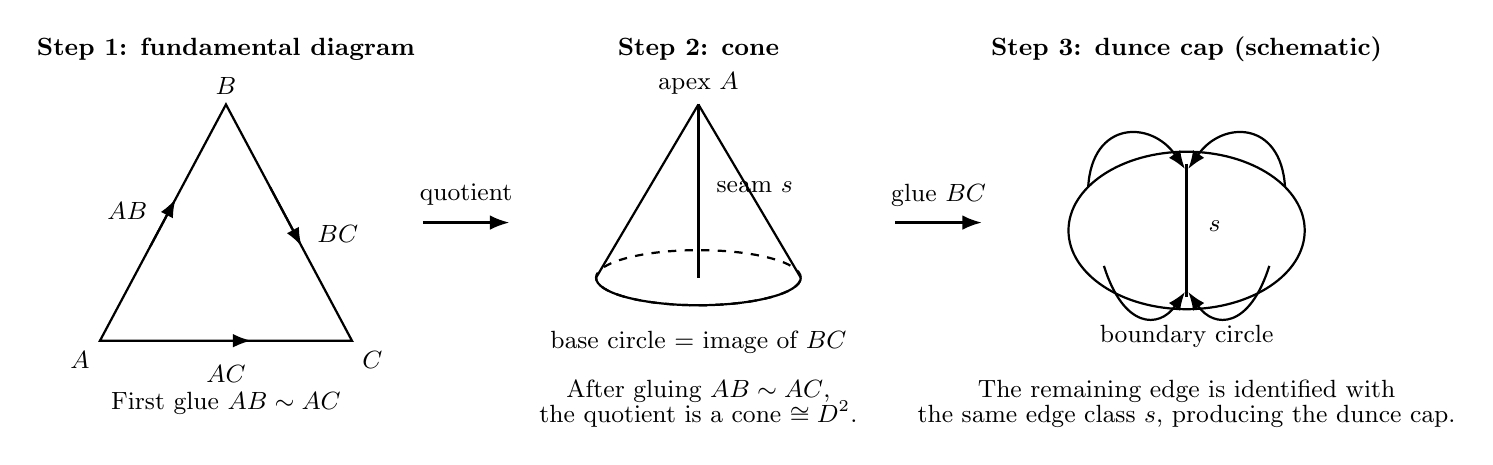
\begin{tikzpicture}[scale=1, >=Latex, thick]
		
		% =========================================================
		% PANEL 1: Fundamental triangle
		% =========================================================
		\begin{scope}[shift={(0,0)}]
			% Title
			\node at (1.6,3.7) {\small\textbf{Step 1: fundamental diagram}};
			
			% Triangle vertices
			\coordinate (A) at (0,0);
			\coordinate (B) at (1.6,3.0);
			\coordinate (C) at (3.2,0);
			
			% Triangle
			\draw (A)--(B)--(C)--cycle;
			
			% Labels
			\node[below left] at (A) {\small \(A\)};
			\node[above] at (B) {\small \(B\)};
			\node[below right] at (C) {\small \(C\)};
			
			% Arrows on edges
			% AB upward
			\draw[->] ($(A)!0.40!(B)$) -- ($(A)!0.60!(B)$);
			% AC from A to C
			\draw[->] ($(A)!0.35!(C)$) -- ($(A)!0.60!(C)$);
			% BC downward
			\draw[->] ($(B)!0.35!(C)$) -- ($(B)!0.60!(C)$);
			
			% Edge labels
			\node[left] at ($(A)!0.55!(B)+(-0.15,0)$) {\small \(AB\)};
			\node[right] at ($(B)!0.55!(C)+(0.15,0)$) {\small \(BC\)};
			\node[below] at ($(A)!0.50!(C)+(0,-0.18)$) {\small \(AC\)};
			
			% Note
			\node[align=center] at (1.6,-0.8) {\small First glue \(AB\sim AC\)};
		\end{scope}
		
		% Arrow between 1 and 2
		\draw[->, line width=0.9pt] (4.1,1.5) -- (5.2,1.5);
		\node at (4.65,1.85) {\small quotient};
		
		% =========================================================
		% PANEL 2: Cone
		% =========================================================
		\begin{scope}[shift={(6,0)}]
			% Title
			\node at (1.6,3.7) {\small\textbf{Step 2: cone}};    
			
			% Cone apex and base
			\coordinate (P) at (1.6,3.0);
			\coordinate (L) at (0.3,0.8);
			\coordinate (R) at (2.9,0.8);
			
			% Base ellipse
			\draw[dashed] (1.6,0.8) ellipse (1.3 and 0.35);
			\draw (0.3,0.8) arc[start angle=180,end angle=360,x radius=1.3,y radius=0.35];
			
			% Side lines
			\draw (P)--(L);
			\draw (P)--(R);
			
			% Seam
			\draw[line width=1pt] (P)--(1.6,0.8);
			\node[right] at (1.7,1.95) {\small seam \(s\)};
			
			% Labels
			\node[above] at (P) {\small apex \(A\)};
			\node[below] at (1.6,0.25) {\small base circle = image of \(BC\)};
			
			% Annotation
			\node[align=center] at (1.6,-0.8)
			{\small After gluing \(AB\sim AC\),\\[-1mm]
				\small the quotient is a cone \(\cong D^2\).};
		\end{scope}
		
		% Arrow between 2 and 3
		\draw[->, line width=0.9pt] (10.1,1.5) -- (11.2,1.5);
		\node at (10.65,1.85) {\small glue \(BC\)};
		
		% =========================================================
		% PANEL 3: Dunce cap schematic
		% =========================================================
		\begin{scope}[shift={(12,0)}]
			% Title
			\node at (1.8,3.7) {\small\textbf{Step 3: dunce cap (schematic)}};
			
			% Disk-like schematic
			\draw (1.8,1.4) ellipse (1.5 and 1.0);
			
			% Boundary circle label
			\node at (1.8,0.05) {\small boundary circle};
			
			% Interior seam
			\draw[line width=1pt] (1.8,2.25)--(1.8,0.55);
			\node[right] at (1.95,1.45) {\small \(s\)};
			
			% Curved arrows showing quotient of boundary onto seam
			\draw[->] (0.55,1.95) .. controls (0.6,2.8) and (1.35,2.8) .. (1.78,2.18);
			\draw[->] (3.05,1.95) .. controls (3.0,2.8) and (2.25,2.8) .. (1.82,2.18);
			\draw[->] (0.75,0.95) .. controls (1.0,0.15) and (1.45,0.15) .. (1.78,0.62);
			\draw[->] (2.85,0.95) .. controls (2.6,0.15) and (2.15,0.15) .. (1.82,0.62);
			
			% Central note
			\node[align=center] at (1.8,-0.8)
			{\small The remaining edge is identified with\\[-1mm]
				\small the same edge class \(s\), producing the dunce cap.};
		\end{scope}
		
	\end{tikzpicture}
	
	\caption{A schematic two-step description of the dunce cap. 
		First one identifies two edges of the triangle, obtaining a cone (hence a disk). 
		Then the remaining edge is glued according to the same orientation rule, which identifies the boundary circle with the existing edge class and yields the dunce cap.}
	\label{fig:dunce-cap-two-step}
\end{figure}


\subsection{\texorpdfstring{Why \(SO(3)\) is not \(S^3\), and how \(SU(2)\) fits in}{Why SO(3) is not S3, and how SU(2) fits in}}

A very common confusion is to identify the rotation group \(SO(3)\) with the \(3\)-sphere \(S^3\).
They are closely related, but they are \emph{not} the same space.

\medskip

\textbf{Key facts.}
\begin{align*}
	SU(2) &\cong S^3,\\
	SO(3) &\cong S^3/\{\pm 1\}\cong \mathbb{RP}^3,\\
	SO(3) &\not\cong S^3.
\end{align*}

Thus the correct picture is that \(S^3\) (equivalently \(SU(2)\)) is a double cover of \(SO(3)\).

\medskip

\textbf{Step 1: \(SU(2)\cong S^3\).}

Recall that
\[
SU(2)=\left\{
\begin{pmatrix}
	a & b\\
	-\overline b & \overline a
\end{pmatrix}
: a,b\in \mathbb C,\ |a|^2+|b|^2=1
\right\}.
\]
So every element of \(SU(2)\) is determined by a pair \((a,b)\in \mathbb C^2\) satisfying
\[
|a|^2+|b|^2=1.
\]
But \(\mathbb C^2\cong \mathbb R^4\), and the equation above is exactly the equation of the unit sphere in \(\mathbb R^4\). Hence, as a manifold,
\[
SU(2)\cong S^3.
\]

\medskip

\textbf{Step 2: \(SU(2)\to SO(3)\) is a \(2\)-to-\(1\) covering map.}

There are several equivalent ways to define this map. One elegant description uses unit quaternions.
Identify \(S^3\) with the unit quaternions
\[
S^3=\{q\in \mathbb H: |q|=1\}.
\]
Then a unit quaternion \(q\) acts on the purely imaginary quaternions
\[
\operatorname{Im}(\mathbb H)\cong \mathbb R^3
\]
by conjugation:
\[
v\longmapsto qvq^{-1}.
\]
This action preserves lengths and orientation, so it defines a rotation of \(\mathbb R^3\). Therefore we get a homomorphism
\[
\Phi:S^3\cong SU(2)\longrightarrow SO(3).
\]
Moreover,
\[
\Phi(q)=\Phi(-q),
\]
and in fact these are the only elements with the same image. Thus the kernel is
\[
\ker(\Phi)=\{\pm 1\},
\]
so \(\Phi\) is a double covering map.

Hence
\[
SO(3)\cong SU(2)/\{\pm I\}\cong S^3/\{\pm 1\}.
\]

\medskip

\textbf{Step 3: why \(SO(3)\neq S^3\).}

They cannot be homeomorphic, because they have different fundamental groups:
\[
\pi_1(S^3)=0,
\qquad
\pi_1(SO(3))\cong \mathbb Z/2\mathbb Z.
\]
Since the fundamental group is a topological invariant, this proves
\[
SO(3)\not\cong S^3.
\]

\medskip

\textbf{Step 4: geometric interpretation of \(SO(3)\).}

A rotation in \(\mathbb R^3\) can be described by:
\begin{itemize}
	\item an axis, given by a unit vector \(u\in S^2\),
	\item an angle \(\theta\in [0,\pi]\).
\end{itemize}
If \(\theta=\pi\), then rotating by angle \(\pi\) around axis \(u\) is the same as rotating by angle \(\pi\) around axis \(-u\). So on the boundary one must identify antipodal points.

This leads to the standard model:
\[
SO(3)\cong \text{closed \(3\)-ball of radius \(\pi\) with antipodal boundary points identified}.
\]
That quotient is homeomorphic to \(\mathbb{RP}^3\), hence
\[
SO(3)\cong \mathbb{RP}^3.
\]

\medskip

\textbf{Step 5: what about \(\mathfrak{so}(3)\)?}

One must also distinguish the Lie group \(SO(3)\) from its Lie algebra \(\mathfrak{so}(3)\).
By definition,
\[
\mathfrak{so}(3)=
\left\{
A\in M_{3\times 3}(\mathbb R): A^T=-A
\right\}.
\]
A general element has the form
\[
\begin{pmatrix}
	0 & -c & b\\
	c & 0 & -a\\
	-b & a & 0
\end{pmatrix},
\qquad a,b,c\in \mathbb R.
\]
So \(\mathfrak{so}(3)\) is a \(3\)-dimensional real vector space, and as a vector space
\[
\mathfrak{so}(3)\cong \mathbb R^3.
\]
Thus:
\begin{itemize}
	\item \(SO(3)\) is a Lie group;
	\item \(S^3\) is a sphere;
	\item \(\mathfrak{so}(3)\) is the tangent Lie algebra at the identity of \(SO(3)\).
\end{itemize}

\medskip

\textbf{Conclusion.}
The precise relationship is
\[
\boxed{
	SU(2)\cong S^3,\qquad
	SO(3)\cong S^3/\{\pm 1\}\cong \mathbb{RP}^3,\qquad
	SO(3)\not\cong S^3.
}
\]

\subsubsection*{Diagram 1: the basic covering picture}

\[
\begin{tikzcd}[column sep=large, row sep=large]
	S^3 \arrow[r, "\cong"] \arrow[dr, two heads, "\;2:1\;"'] & SU(2) \arrow[d, two heads, "\Phi"] \\
	& SO(3)
\end{tikzcd}
\]

Since \(\ker(\Phi)=\{\pm I\}\), one also has
\[
SO(3)\cong SU(2)/\{\pm I\}\cong S^3/\{\pm 1\}.
\]

\subsubsection*{Diagram 2: ball model of \texorpdfstring{\(SO(3)\)}{SO(3)}}

\begin{center}
	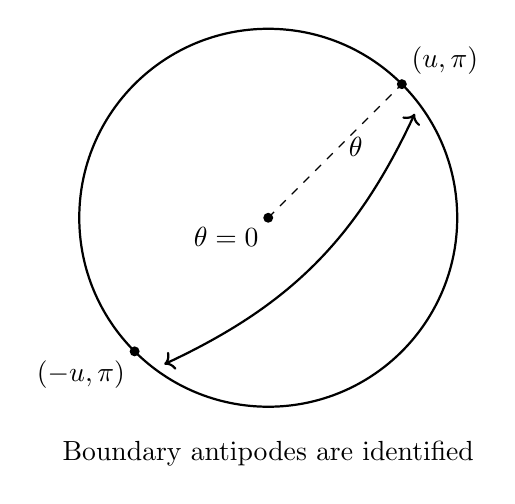
\begin{tikzpicture}[scale=1.2]
		% Ball
		\draw[thick] (0,0) circle (2);
		
		% Center
		\fill (0,0) circle (1.5pt);
		\node[below left] at (0,0) {\(\theta=0\)};
		
		% Radius
		\draw[dashed] (0,0) -- (1.4,1.4);
		\node[right] at (0.75,0.75) {\(\theta\)};
		
		% Boundary labels
		\fill (1.414,1.414) circle (1.5pt);
		\fill (-1.414,-1.414) circle (1.5pt);
		\node[above right] at (1.414,1.414) {\((u,\pi)\)};
		\node[below left] at (-1.414,-1.414) {\((-u,\pi)\)};
		
		% Arrow showing identification
		\draw[<->, thick] (1.55,1.1) to[bend left=20] (-1.1,-1.55);
		\node at (0,-2.5) {Boundary antipodes are identified};
	\end{tikzpicture}
\end{center}

This picture means: each interior point represents a rotation by angle \(\theta\in(0,\pi)\) about some axis \(u\), while opposite boundary points represent the same rotation by angle \(\pi\).

\subsubsection*{Optional diagram 3: quotient viewpoint}

\[
\begin{tikzcd}[column sep=huge]
	S^3 \arrow[r, two heads] & S^3/\{\pm1\} \arrow[r, "\cong"] & \mathbb{RP}^3 \arrow[r, "\cong"] & SO(3)
\end{tikzcd}
\]

\subsection{\texorpdfstring{Dimension of \(S^3\), \(SO(3)\), and the axis--angle description}{Dimension of S3, SO(3), and the axis-angle description}}

It is important to distinguish between:

\begin{itemize}
	\item the sphere \(S^3\),
	\item the rotation group \(SO(3)\),
	\item the Lie algebra \(\mathfrak{so}(3)\).
\end{itemize}

Although these objects are closely related, they are not the same thing.  
In particular, both \(S^3\) and \(SO(3)\) are \(3\)-dimensional manifolds, but for different reasons.

\subsubsection*{1. The dimension of \texorpdfstring{\(S^3\)}{S3}}

By definition,
\[
S^3=\{(x_1,x_2,x_3,x_4)\in \mathbb R^4 : x_1^2+x_2^2+x_3^2+x_4^2=1\}.
\]
So \(S^3\) is the unit sphere in \(\mathbb R^4\).

\medskip

\textbf{Important point:}
\begin{itemize}
	\item \(S^3\) lives inside \(\mathbb R^4\),
	\item but its intrinsic dimension is \(3\).
\end{itemize}

This is exactly analogous to:
\[
S^1\subset \mathbb R^2,\qquad S^2\subset \mathbb R^3,\qquad S^3\subset \mathbb R^4.
\]
In general, \(S^n\) is an \(n\)-dimensional manifold sitting inside \(\mathbb R^{n+1}\).

So:
\[
\boxed{\dim S^3=3.}
\]

\subsubsection*{2. The dimension of \texorpdfstring{\(SO(3)\)}{SO(3)}}

The group \(SO(3)\) is the group of orientation-preserving orthogonal linear maps of \(\mathbb R^3\), that is,
\[
SO(3)=\{A\in M_{3\times 3}(\mathbb R): A^TA=I,\ \det A=1\}.
\]

Geometrically, an element of \(SO(3)\) is a rotation of \(\mathbb R^3\).

A rotation can be described by:
\begin{itemize}
	\item an axis of rotation,
	\item an angle of rotation.
\end{itemize}

At first sight one might think:
\begin{quote}
	``The axis is a vector in \(\mathbb R^3\), so it should contribute \(3\) dimensions, and the angle contributes \(1\), hence \(4\).''
\end{quote}
But this is \emph{not} correct, because an axis is not an arbitrary vector: it is only a \emph{direction}.

\subsubsection*{3. Why the axis contributes only \texorpdfstring{\(2\)}{2} dimensions}

To specify a direction in \(\mathbb R^3\), we may choose a unit vector
\[
u\in S^2=\{(x,y,z)\in \mathbb R^3 : x^2+y^2+z^2=1\}.
\]
The set \(S^2\) is \(2\)-dimensional, so the axis contributes \(2\) parameters.

Another way to say the same thing is this:

\begin{itemize}
	\item a general vector in \(\mathbb R^3\) has \(3\) coordinates;
	\item requiring it to have length \(1\) imposes one equation,
	\[
	x^2+y^2+z^2=1,
	\]
	so one degree of freedom is lost.
\end{itemize}

Therefore:
\[
3-1=2.
\]

So the axis does \emph{not} contribute \(3\) dimensions. It contributes only \(2\).

\[
\boxed{\text{axis direction} \in S^2 \quad \Longrightarrow \quad 2\text{ dimensions}.}
\]

\subsubsection*{4. The angle contributes \texorpdfstring{\(1\)}{1} dimension}

Once the axis is fixed, we choose an angle \(\theta\).  
This is just one real parameter.

For example, one may take
\[
\theta\in [0,2\pi)
\]
or, if one wants a more symmetric geometric description, one may take
\[
0\le \theta\le \pi
\]
with suitable identifications.

In either case, the angle contributes exactly one degree of freedom.

\[
\boxed{\text{angle } \theta \quad \Longrightarrow \quad 1\text{ dimension}.}
\]

\subsubsection*{5. Therefore \texorpdfstring{\(SO(3)\)}{SO(3)} is \texorpdfstring{\(3\)}{3}-dimensional}

Combining the axis and the angle gives:
\[
\dim SO(3)=2+1=3.
\]

So the correct dimension count is
\[
\boxed{\dim SO(3)=3.}
\]

\medskip

\textbf{Important correction.}  
The sphere \(S^2\) describes the \emph{axis}, not the angle.  
The angle is a single real parameter, not a point of \(S^2\).

\subsubsection*{6. A more geometric model: the closed ball}

A very useful way to visualize \(SO(3)\) is by the \emph{axis--angle ball model}.

Let \(u\in S^2\) be the axis and \(0\le \theta\le \pi\) the angle.  
Associate to the rotation the vector
\[
x=\theta u\in \mathbb R^3.
\]
Then \(\|x\|=\theta\), so \(x\) lies in the closed ball of radius \(\pi\):
\[
B_\pi^3=\{x\in \mathbb R^3 : \|x\|\le \pi\}.
\]

In this model:

\begin{itemize}
	\item the center \(x=0\) corresponds to the identity rotation;
	\item interior points \(0<\|x\|<\pi\) correspond to rotations by angle \(0<\theta<\pi\);
	\item boundary points \(\|x\|=\pi\) correspond to rotations by angle \(\pi\).
\end{itemize}

Now comes the key identification:

rotating by angle \(\pi\) about axis \(u\) is the same as rotating by angle \(\pi\) about axis \(-u\).

Therefore opposite boundary points represent the same rotation, so we must identify antipodal points on the boundary:
\[
x\sim -x \qquad \text{for } x\in \partial B_\pi^3.
\]

Hence one gets the quotient model
\[
\boxed{
	SO(3)\cong B_\pi^3/\bigl(x\sim -x \text{ on } \partial B_\pi^3\bigr).
}
\]

This is another way to see that \(SO(3)\) is \(3\)-dimensional.

\subsubsection*{7. Relation with \texorpdfstring{\(S^3\)}{S3}}

Although \(SO(3)\) is \(3\)-dimensional, it is \emph{not} the same space as \(S^3\).

The correct relation is:
\[
SU(2)\cong S^3,
\qquad
SO(3)\cong S^3/\{\pm 1\}\cong \mathbb{RP}^3.
\]

So \(S^3\) is a double cover of \(SO(3)\), but not equal to it.

In particular,
\[
\pi_1(S^3)=0,
\qquad
\pi_1(SO(3))\cong \mathbb Z/2\mathbb Z,
\]
so these spaces cannot be homeomorphic.

\subsubsection*{8. What about \texorpdfstring{\(\mathfrak{so}(3)\)}{so(3)}?}

The Lie algebra \(\mathfrak{so}(3)\) is the space of skew-symmetric \(3\times 3\) matrices:
\[
\mathfrak{so}(3)=\{A\in M_{3\times 3}(\mathbb R): A^T=-A\}.
\]
A general element has the form
\[
\begin{pmatrix}
	0 & -c & b\\
	c & 0 & -a\\
	-b & a & 0
\end{pmatrix},
\qquad a,b,c\in \mathbb R.
\]
So \(\mathfrak{so}(3)\) depends on three real parameters and therefore
\[
\boxed{\dim \mathfrak{so}(3)=3.}
\]

Thus:
\begin{itemize}
	\item \(S^3\) is a \(3\)-dimensional sphere in \(\mathbb R^4\),
	\item \(SO(3)\) is a \(3\)-dimensional Lie group of rotations,
	\item \(\mathfrak{so}(3)\) is a \(3\)-dimensional Lie algebra.
\end{itemize}

\subsubsection*{9. Final summary}

\[
\boxed{
	\dim S^3=3,\qquad \dim SO(3)=3,\qquad \dim \mathfrak{so}(3)=3.
}
\]

But these dimensions come from different geometric descriptions:

\begin{itemize}
	\item \(S^3\) is defined by one equation inside \(\mathbb R^4\);
	\item \(SO(3)\) comes from \((\text{axis direction})+(\text{angle})=2+1\);
	\item \(\mathfrak{so}(3)\) is a \(3\)-dimensional vector space of skew-symmetric matrices.
\end{itemize}

\subsubsection*{Diagram 1: axis contributes \(2\), angle contributes \(1\)}

\begin{center}
	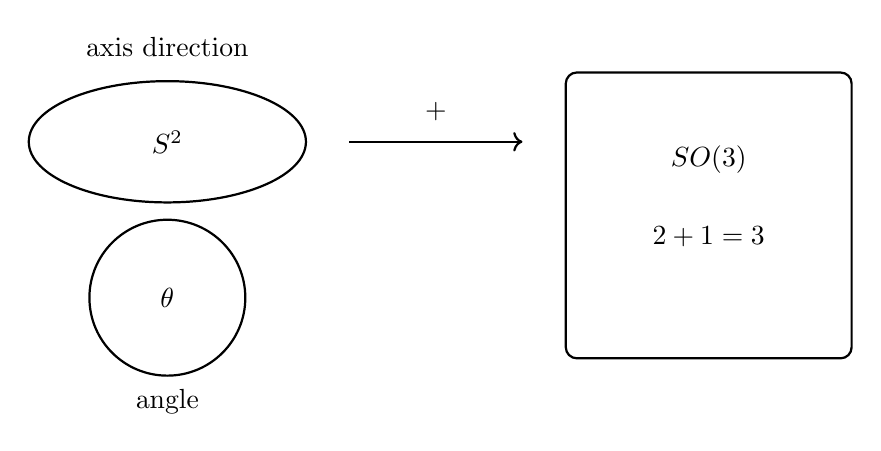
\begin{tikzpicture}[scale=1.1]
		\draw[thick] (0,0) ellipse (1.6 and 0.7);
		\draw[thick] (0,-1.8) circle (0.9);
		
		\node at (0,0) {\(S^2\)};
		\node at (0,-1.8) {\(\theta\)};
		
		\draw[->, thick] (2.1,0) -- (4.1,0);
		\node at (3.1,0.35) {\(+\)};
		
		\draw[rounded corners, thick] (4.6,0.8) rectangle (7.9,-2.5);
		\node at (6.25,-0.2) {\(SO(3)\)};
		\node at (6.25,-1.1) {\(2+1=3\)};
		
		\node at (0,1.1) {axis direction};
		\node at (0,-3.0) {angle};
	\end{tikzpicture}
\end{center}

\subsubsection*{Diagram 2: the ball model of \texorpdfstring{\(SO(3)\)}{SO(3)}}

\begin{center}
	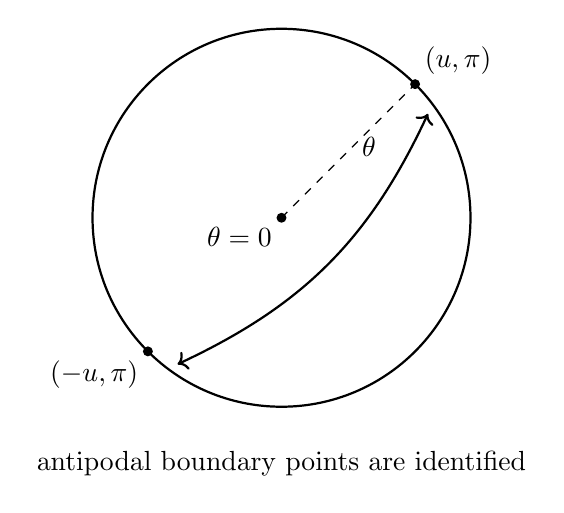
\begin{tikzpicture}[scale=1.2]
		\draw[thick] (0,0) circle (2);
		
		\fill (0,0) circle (1.5pt);
		\node[below left] at (0,0) {\(\theta=0\)};
		
		\draw[dashed] (0,0) -- (1.4,1.4);
		\node[right] at (0.75,0.75) {\(\theta\)};
		
		\fill (1.414,1.414) circle (1.5pt);
		\fill (-1.414,-1.414) circle (1.5pt);
		
		\node[above right] at (1.414,1.414) {\((u,\pi)\)};
		\node[below left] at (-1.414,-1.414) {\((-u,\pi)\)};
		
		\draw[<->, thick] (1.55,1.1) to[bend left=20] (-1.1,-1.55);
		
		\node at (0,-2.6) {antipodal boundary points are identified};
	\end{tikzpicture}
\end{center}

So the ball itself is \(3\)-dimensional, and the quotient identification occurs only on its boundary. This gives another geometric model of the \(3\)-dimensional manifold \(SO(3)\).

\end{document}
